
%% bare_jrnl.tex
%% V1.4b
%% 2015/08/26
%% by Michael Shell
%% see http://www.michaelshell.org/
%% for current contact information.
%%
%% This is a skeleton file demonstrating the use of IEEEtran.cls
%% (requires IEEEtran.cls version 1.8b or later) with an IEEE
%% journal paper.
%%
%% Support sites:
%% http://www.michaelshell.org/tex/ieeetran/
%% http://www.ctan.org/pkg/ieeetran
%% and
%% http://www.ieee.org/

%%*************************************************************************
%% Legal Notice:
%% This code is offered as-is without any warranty either expressed or
%% implied; without even the implied warranty of MERCHANTABILITY or
%% FITNESS FOR A PARTICULAR PURPOSE!
%% User assumes all risk.
%% In no event shall the IEEE or any contributor to this code be liable for
%% any damages or losses, including, but not limited to, incidental,
%% consequential, or any other damages, resulting from the use or misuse
%% of any information contained here.
%%
%% All comments are the opinions of their respective authors and are not
%% necessarily endorsed by the IEEE.
%%
%% This work is distributed under the LaTeX Project Public License (LPPL)
%% ( http://www.latex-project.org/ ) version 1.3, and may be freely used,
%% distributed and modified. A copy of the LPPL, version 1.3, is included
%% in the base LaTeX documentation of all distributions of LaTeX released
%% 2003/12/01 or later.
%% Retain all contribution notices and credits.
%% ** Modified files should be clearly indicated as such, including  **
%% ** renaming them and changing author support contact information. **
%%*************************************************************************


% *** Authors should verify (and, if needed, correct) their LaTeX system  ***
% *** with the testflow diagnostic prior to trusting their LaTeX platform ***
% *** with production work. The IEEE's font choices and paper sizes can   ***
% *** trigger bugs that do not appear when using other class files.       ***                          ***
% The testflow support page is at:
% http://www.michaelshell.org/tex/testflow/

%\documentclass[onecolumn]{IEEEtran}
%\linespread{2.0}
\documentclass[journal]{IEEEtran}
%
% If IEEEtran.cls has not been installed into the LaTeX system files,
% manually specify the path to it like:
% \documentclass[journal]{../sty/IEEEtran}




% Some very useful LaTeX packages include:
% (uncomment the ones you want to load)


% *** MISC UTILITY PACKAGES ***
%
%\usepackage{ifpdf}
% Heiko Oberdiek's ifpdf.sty is very useful if you need conditional
% compilation based on whether the output is pdf or dvi.
% usage:
% \ifpdf
%   % pdf code
% \else
%   % dvi code
% \fi
% The latest version of ifpdf.sty can be obtained from:
% http://www.ctan.org/pkg/ifpdf
% Also, note that IEEEtran.cls V1.7 and later provides a builtin
% \ifCLASSINFOpdf conditional that works the same way.
% When switching from latex to pdflatex and vice-versa, the compiler may
% have to be run twice to clear warning/error messages.
\usepackage{graphics}
\usepackage{graphicx}
\usepackage{epsfig}
\usepackage{subfigure}
\usepackage{tikz}
\usepackage{lineno}
\usepackage{amssymb}
\usepackage{amsmath}
\usepackage{epsfig}
\usepackage{rotating}
\usepackage[hang,stable]{footmisc}
\usepackage{color}
\usepackage{bm}
\usepackage{multirow}
\usepackage{dcolumn}
\usepackage{booktabs}
\usepackage{ifpdf}
\usepackage{amsthm}
\usepackage{CJK}
\usepackage{cases,setspace}
\usepackage{setspace}
\usepackage{float}
\usepackage{graphicx}
\usepackage{subfigure}
\usepackage{listings}
\usepackage{epstopdf}
\usepackage{cite}
\usepackage{bbm}
\newtheorem{theorem}{Theorem}
\newtheorem{corollary}[theorem]{Corollary}
\newtheorem{proposition}[theorem]{Proposition}
\newtheorem{lemma}{Lemma}
%\theoremstyle{definition}
\newtheorem{definition}{Definition}
\newtheorem{remark}{Remark}
\newtheorem*{problem0}{Problem P$_0$}
\newtheorem*{problemN}{Problem P$_N$}
\newtheorem*{problemP}{Problem P$_1$}
\newtheorem*{problemQ}{Problem P$_2$}
% *** CITATION PACKAGES ***
%
%\usepackage{cite}
% cite.sty was written by Donald Arseneau
% V1.6 and later of IEEEtran pre-defines the format of the cite.sty package
% \cite{} output to follow that of the IEEE. Loading the cite package will
% result in citation numbers being automatically sorted and properly
% "compressed/ranged". e.g., [1], [9], [2], [7], [5], [6] without using
% cite.sty will become [1], [2], [5]--[7], [9] using cite.sty. cite.sty's
% \cite will automatically add leading space, if needed. Use cite.sty's
% noadjust option (cite.sty V3.8 and later) if you want to turn this off
% such as if a citation ever needs to be enclosed in parenthesis.
% cite.sty is already installed on most LaTeX systems. Be sure and use
% version 5.0 (2009-03-20) and later if using hyperref.sty.
% The latest version can be obtained at:
% http://www.ctan.org/pkg/cite
% The documentation is contained in the cite.sty file itself.






% *** GRAPHICS RELATED PACKAGES ***
%
\ifCLASSINFOpdf
  % \usepackage[pdftex]{graphicx}
  % declare the path(s) where your graphic files are
  % \graphicspath{{../pdf/}{../jpeg/}}
  % and their extensions so you won't have to specify these with
  % every instance of \includegraphics
  % \DeclareGraphicsExtensions{.pdf,.jpeg,.png}
\else
  % or other class option (dvipsone, dvipdf, if not using dvips). graphicx
  % will default to the driver specified in the system graphics.cfg if no
  % driver is specified.
  % \usepackage[dvips]{graphicx}
  % declare the path(s) where your graphic files are
  % \graphicspath{{../eps/}}
  % and their extensions so you won't have to specify these with
  % every instance of \includegraphics
  % \DeclareGraphicsExtensions{.eps}
\fi
% graphicx was written by David Carlisle and Sebastian Rahtz. It is
% required if you want graphics, photos, etc. graphicx.sty is already
% installed on most LaTeX systems. The latest version and documentation
% can be obtained at:
% http://www.ctan.org/pkg/graphicx
% Another good source of documentation is "Using Imported Graphics in
% LaTeX2e" by Keith Reckdahl which can be found at:
% http://www.ctan.org/pkg/epslatex
%
% latex, and pdflatex in dvi mode, support graphics in encapsulated
% postscript (.eps) format. pdflatex in pdf mode supports graphics
% in .pdf, .jpeg, .png and .mps (metapost) formats. Users should ensure
% that all non-photo figures use a vector format (.eps, .pdf, .mps) and
% not a bitmapped formats (.jpeg, .png). The IEEE frowns on bitmapped formats
% which can result in "jaggedy"/blurry rendering of lines and letters as
% well as large increases in file sizes.
%
% You can find documentation about the pdfTeX application at:
% http://www.tug.org/applications/pdftex





% *** MATH PACKAGES ***
%
%\usepackage{amsmath}
% A popular package from the American Mathematical Society that provides
% many useful and powerful commands for dealing with mathematics.
%
% Note that the amsmath package sets \interdisplaylinepenalty to 10000
% thus preventing page breaks from occurring within multiline equations. Use:
%\interdisplaylinepenalty=2500
% after loading amsmath to restore such page breaks as IEEEtran.cls normally
% does. amsmath.sty is already installed on most LaTeX systems. The latest
% version and documentation can be obtained at:
% http://www.ctan.org/pkg/amsmath





% *** SPECIALIZED LIST PACKAGES ***
%
%\usepackage{algorithmic}
% algorithmic.sty was written by Peter Williams and Rogerio Brito.
% This package provides an algorithmic environment fo describing algorithms.
% You can use the algorithmic environment in-text or within a figure
% environment to provide for a floating algorithm. Do NOT use the algorithm
% floating environment provided by algorithm.sty (by the same authors) or
% algorithm2e.sty (by Christophe Fiorio) as the IEEE does not use dedicated
% algorithm float types and packages that provide these will not provide
% correct IEEE style captions. The latest version and documentation of
% algorithmic.sty can be obtained at:
% http://www.ctan.org/pkg/algorithms
% Also of interest may be the (relatively newer and more customizable)
% algorithmicx.sty package by Szasz Janos:
% http://www.ctan.org/pkg/algorithmicx




% *** ALIGNMENT PACKAGES ***
%
%\usepackage{array}
% Frank Mittelbach's and David Carlisle's array.sty patches and improves
% the standard LaTeX2e array and tabular environments to provide better
% appearance and additional user controls. As the default LaTeX2e table
% generation code is lacking to the point of almost being broken with
% respect to the quality of the end results, all users are strongly
% advised to use an enhanced (at the very least that provided by array.sty)
% set of table tools. array.sty is already installed on most systems. The
% latest version and documentation can be obtained at:
% http://www.ctan.org/pkg/array


% IEEEtran contains the IEEEeqnarray family of commands that can be used to
% generate multiline equations as well as matrices, tables, etc., of high
% quality.




% *** SUBFIGURE PACKAGES ***
%\ifCLASSOPTIONcompsoc
%  \usepackage[caption=false,font=normalsize,labelfont=sf,textfont=sf]{subfig}
%\else
%  \usepackage[caption=false,font=footnotesize]{subfig}
%\fi
% subfig.sty, written by Steven Douglas Cochran, is the modern replacement
% for subfigure.sty, the latter of which is no longer maintained and is
% incompatible with some LaTeX packages including fixltx2e. However,
% subfig.sty requires and automatically loads Axel Sommerfeldt's caption.sty
% which will override IEEEtran.cls' handling of captions and this will result
% in non-IEEE style figure/table captions. To prevent this problem, be sure
% and invoke subfig.sty's "caption=false" package option (available since
% subfig.sty version 1.3, 2005/06/28) as this is will preserve IEEEtran.cls
% handling of captions.
% Note that the Computer Society format requires a larger sans serif font
% than the serif footnote size font used in traditional IEEE formatting
% and thus the need to invoke different subfig.sty package options depending
% on whether compsoc mode has been enabled.
%
% The latest version and documentation of subfig.sty can be obtained at:
% http://www.ctan.org/pkg/subfig




% *** FLOAT PACKAGES ***
%
%\usepackage{fixltx2e}
% fixltx2e, the successor to the earlier fix2col.sty, was written by
% Frank Mittelbach and David Carlisle. This package corrects a few problems
% in the LaTeX2e kernel, the most notable of which is that in current
% LaTeX2e releases, the ordering of single and double column floats is not
% guaranteed to be preserved. Thus, an unpatched LaTeX2e can allow a
% single column figure to be placed prior to an earlier double column
% figure.
% Be aware that LaTeX2e kernels dated 2015 and later have fixltx2e.sty's
% corrections already built into the system in which case a warning will
% be issued if an attempt is made to load fixltx2e.sty as it is no longer
% needed.
% The latest version and documentation can be found at:
% http://www.ctan.org/pkg/fixltx2e


%\usepackage{stfloats}
% stfloats.sty was written by Sigitas Tolusis. This package gives LaTeX2e
% the ability to do double column floats at the bottom of the page as well
% as the top. (e.g., "\begin{figure*}[!b]" is not normally possible in
% LaTeX2e). It also provides a command:
%\fnbelowfloat
% to enable the placement of footnotes below bottom floats (the standard
% LaTeX2e kernel puts them above bottom floats). This is an invasive package
% which rewrites many portions of the LaTeX2e float routines. It may not work
% with other packages that modify the LaTeX2e float routines. The latest
% version and documentation can be obtained at:
% http://www.ctan.org/pkg/stfloats
% Do not use the stfloats baselinefloat ability as the IEEE does not allow
% \baselineskip to stretch. Authors submitting work to the IEEE should note
% that the IEEE rarely uses double column equations and that authors should try
% to avoid such use. Do not be tempted to use the cuted.sty or midfloat.sty
% packages (also by Sigitas Tolusis) as the IEEE does not format its papers in
% such ways.
% Do not attempt to use stfloats with fixltx2e as they are incompatible.
% Instead, use Morten Hogholm'a dblfloatfix which combines the features
% of both fixltx2e and stfloats:
%
% \usepackage{dblfloatfix}
% The latest version can be found at:
% http://www.ctan.org/pkg/dblfloatfix




%\ifCLASSOPTIONcaptionsoff
%  \usepackage[nomarkers]{endfloat}
% \let\MYoriglatexcaption\caption
% \renewcommand{\caption}[2][\relax]{\MYoriglatexcaption[#2]{#2}}
%\fi
% endfloat.sty was written by James Darrell McCauley, Jeff Goldberg and
% Axel Sommerfeldt. This package may be useful when used in conjunction with
% IEEEtran.cls'  captionsoff option. Some IEEE journals/societies require that
% submissions have lists of figures/tables at the end of the paper and that
% figures/tables without any captions are placed on a page by themselves at
% the end of the document. If needed, the draftcls IEEEtran class option or
% \CLASSINPUTbaselinestretch interface can be used to increase the line
% spacing as well. Be sure and use the nomarkers option of endfloat to
% prevent endfloat from "marking" where the figures would have been placed
% in the text. The two hack lines of code above are a slight modification of
% that suggested by in the endfloat docs (section 8.4.1) to ensure that
% the full captions always appear in the list of figures/tables - even if
% the user used the short optional argument of \caption[]{}.
% IEEE papers do not typically make use of \caption[]'s optional argument,
% so this should not be an issue. A similar trick can be used to disable
% captions of packages such as subfig.sty that lack options to turn off
% the subcaptions:
% For subfig.sty:
% \let\MYorigsubfloat\subfloat
% \renewcommand{\subfloat}[2][\relax]{\MYorigsubfloat[]{#2}}
% However, the above trick will not work if both optional arguments of
% the \subfloat command are used. Furthermore, there needs to be a
% description of each subfigure *somewhere* and endfloat does not add
% subfigure captions to its list of figures. Thus, the best approach is to
% avoid the use of subfigure captions (many IEEE journals avoid them anyway)
% and instead reference/explain all the subfigures within the main caption.
% The latest version of endfloat.sty and its documentation can obtained at:
% http://www.ctan.org/pkg/endfloat
%
% The IEEEtran \ifCLASSOPTIONcaptionsoff conditional can also be used
% later in the document, say, to conditionally put the References on a
% page by themselves.




% *** PDF, URL AND HYPERLINK PACKAGES ***
%
%\usepackage{url}
% url.sty was written by Donald Arseneau. It provides better support for
% handling and breaking URLs. url.sty is already installed on most LaTeX
% systems. The latest version and documentation can be obtained at:
% http://www.ctan.org/pkg/url
% Basically, \url{my_url_here}.




% *** Do not adjust lengths that control margins, column widths, etc. ***
% *** Do not use packages that alter fonts (such as pslatex).         ***
% There should be no need to do such things with IEEEtran.cls V1.6 and later.
% (Unless specifically asked to do so by the journal or conference you plan
% to submit to, of course. )


% correct bad hyphenation here
\hyphenation{op-tical net-works semi-conduc-tor}


\begin{document}
%
% paper title
% Titles are generally capitalized except for words such as a, an, and, as,
% at, but, by, for, in, nor, of, on, or, the, to and up, which are usually
% not capitalized unless they are the first or last word of the title.
% Linebreaks \\ can be used within to get better formatting as desired.
% Do not put math or special symbols in the title.
\title{Fast Linear Parameter Varying Model Predictive Control of Buck DC-DC Converters Based on FPGA}
%
%
% author names and IEEE memberships
% note positions of commas and nonbreaking spaces ( ~ ) LaTeX will not break
% a structure at a ~ so this keeps an author's name from being broken across
% two lines.
% use \thanks{} to gain access to the first footnote area
% a separate \thanks must be used for each paragraph as LaTeX2e's \thanks
% was not built to handle multiple paragraphs
%

\author{Zhen Liu, Lei Xie,\emph{~Member,~IEEE}, Alberto Bemporad,\emph{~Fellow,~IEEE}% <-this % stops a space

\thanks{
This work was supported by National Key R\&D Program of
China(Grant No. 2018YFF0214701), Natural Science Foundation of China
(Grant Nos. 61673358 and 61621002) and Natural Science Foundation of
Zhejiang, China (No. LR17F030002).\emph{Corresponding author: Lei Xie.}
	
Zhen Liu and Lei Xie are with State Key Laboratory of Industrial Control Technology, Zhejiang University, 310027 Hangzhou, China. (email: 3090101109@zju.edu.cn; leix@iipc.zju.edu.cn). 

Alberto Bemporad is with IMT School for Advanced Studies, Lucca, Italy (email: alberto.bemporad@imtlucca.it)}% <-this % stops a space

%\thanks{Manuscript received April 19, 2005; revised August 26, 2015.}
}

% note the % following the last \IEEEmembership and also \thanks -
% these prevent an unwanted space from occurring between the last author name
% and the end of the author line. i.e., if you had this:
%
% \author{....lastname \thanks{...} \thanks{...} }
%                     ^------------^------------^----Do not want these spaces!
%
% a space would be appended to the last name and could cause every name on that
% line to be shifted left slightly. This is one of those "LaTeX things". For
% instance, "\textbf{A} \textbf{B}" will typeset as "A B" not "AB". To get
% "AB" then you have to do: "\textbf{A}\textbf{B}"
% \thanks is no different in this regard, so shield the last } of each \thanks
% that ends a line with a % and do not let a space in before the next \thanks.
% Spaces after \IEEEmembership other than the last one are OK (and needed) as
% you are supposed to have spaces between the names. For what it is worth,
% this is a minor point as most people would not even notice if the said evil
% space somehow managed to creep in.



% The paper headers
%\markboth{Journal of \LaTeX\ Class Files,~Vol.~14, No.~8, August~2015}%
%{Shell \MakeLowercase{\textit{et al.}}: Bare Demo of IEEEtran.cls for IEEE Journals}
% The only time the second header will appear is for the odd numbered pages
% after the title page when using the twoside option.
%
% *** Note that you probably will NOT want to include the author's ***
% *** name in the headers of peer review papers.                   ***
% You can use \ifCLASSOPTIONpeerreview for conditional compilation here if
% you desire.




% If you want to put a publisher's ID mark on the page you can do it like
% this:
%\IEEEpubid{0000--0000/00\$00.00~\copyright~2015 IEEE}
% Remember, if you use this you must call \IEEEpubidadjcol in the second
% column for its text to clear the IEEEpubid mark.



% use for special paper notices
%\IEEEspecialpapernotice{(Invited Paper)}




% make the title area
\maketitle

% As a general rule, do not put math, special symbols or citations
% in the abstract or keywords.
\begin{abstract}
This paper introduces a novel fast model predictive control (MPC) methodology based on linear parameter varying (LPV) systems. The proposed approach can deal with large-scale problems better than conventional fast MPC methods. First the equality constraints given by the model equations are not eliminated to get a condensed quadratic programming (QP) problem, as the model of the LPV system changes and it will be time-consuming to reformulate the QP problem at each sampling time. Instead, the proposed approach constructs a sparse QP problem by keeping the equality constraints. Although the resulting QP problem has larger dimension than the condensed one, it can be reformulated and solved as a system of piecewise affine (PWA) equations given by the Karush-Kuhn-Tucker (KKT) conditions of optimality. Finally the problem will be solved through a Newton-method and an exact line search in a fast way. The performance is tested and compared with off-the-shelf QP solvers on the conventional buck DC-DC converter control problem both in simulations and the experiments on FPGA. The proposed methodology works well for the controller and is especially faster in comparison with some other conventional algorithms for large prediction horizons.
\end{abstract}

% Note that keywords are not normally used for peerreview papers.
\begin{IEEEkeywords}
buck DC-DC converter, linear parameter varying, model predictive control, non-condensed quadratic programming problem
\end{IEEEkeywords}


% For peer review papers, you can put extra information on the cover
% page as needed:
% \ifCLASSOPTIONpeerreview
% \begin{center} \bfseries EDICS Category: 3-BBND \end{center}
% \fi
%
% For peerreview papers, this IEEEtran command inserts a page break and
% creates the second title. It will be ignored for other modes.
\IEEEpeerreviewmaketitle

\section{INTRODUCTION}
% The very first letter is a 2 line initial drop letter followed
% by the rest of the first word in caps.
%
% form to use if the first word consists of a single letter:
% \IEEEPARstart{A}{demo} file is ....
%
% form to use if you need the single drop letter followed by
% normal text (unknown if ever used by the IEEE):
% \IEEEPARstart{A}{}demo file is ....
%
% Some journals put the first two words in caps:
% \IEEEPARstart{T}{his demo} file is ....
%
% Here we have the typical use of a "T" for an initial drop letter
% and "HIS" in caps to complete the first word.
\IEEEPARstart
Model predictive control (MPC) owes its advantages to the characteristic that can stabilize linear or nonlinear systems subject to hard input and state constraints \cite{mayne2000constrained}. For the simpler use of linear systems subject to linear constraints, the resulting optimal control problem can be reformulated as a ``condensed'' quadratic programming (QP) problem by eliminating the equality constraints reformed by the dynamic model of the system, and off-the-shelf QP solvers support the application of MPC for small-scale to medium-scale processes \cite{rawlings2009model}. Meanwhile, when implementing such MPC methods to linear parameter varying (LPV) systems, such as to control nonlinear systems with real-time linearization it is necessary to reformulate the QP problem at each sampling time because the model is changing. However, the repeated multiplication of the coefficient matrices to get the condensed QP problem \cite{richards2015fast} may require substantial computation effort and meet the bottleneck of the methodology. Especially for high sampling rates and large-scale systems, the computation time for constructing the QP problem may become a limiting factor. The present work constructs a sparse non-condensed QP problem by keeping the equality constraints in the formulation \cite{rubagotti2014stabilizing} and apply a piecewise smooth Newton algorithm developed in \cite{li1997new} combined with Cholesky factorization and exact line search to maintain small computation time \cite{patrinos2011global} regardless of the increasing dimension of the problem.

Our goal is to adopt MPC and its intrinsic capacity of handling constraints beyond slow dynamic systems, in particular to systems with high sampling rates such as power electronic converters. Experiments on controlling DC-DC converters by MPC are repeated in \cite{geyer2008hybrid} showing that online MPC is possible for fast systems. During the last years many good algorithms have been developed for high speed MPC such as active-set methods \cite{ferreau2008online}, interior-point methods \cite{mattingley2012cvxgen} and fast-gradient methods \cite{richter2009real} and packages for QP are increasingly becoming the core of solving MPC problems fast enough to fulfill the real-time requirements. Recently online optimization provides several novel concepts of solving QP in a fast way. \cite{wang2010fast} proposes a sparse MPC structure and uses the Cholesky factorization so that the Newton-method can be solved  in low flops. And \cite{richter2012computational} provides the idea of fast solvers based on the KKT condition. The algorithm of this paper utilizes these ideas synthetically.

A switching converter system can be stable around the operating point, however, it may be unstable when the system meets parameters varying \cite{vlad2014advanced} \cite{olalla2012robust}. In order to take parameter uncertainty into consideration, the study of how to set up the converter models is still a significant field of investigation \cite{olalla2009robust}. This paper presents a linear design method based on a developed LPV representation of the buck DC-DC converter \cite{thabet2016set} in order to achieve robust stability and performance when model inaccuracies happen.

In recent works, \cite{dehghanzadeh2018model,kumar2014comparison,gaouzi2017constrained} present a conventional MPC controller which contains the transition from MPC to condensed QP and an off-the-shelf QP solver. Meanwhile \cite{vazquez2017model} summarizes that the recent literatures on MPC of power converters mainly concern the prediction model, the cost function and optimization algorithm. These works propose approaches for better prediction model of the converter, for more appropriate cost function selection that can match closely to the type of the power converter, for better design of the weighting factor that is rather important in MPC construction. Finally, about the optimization algorithm issues, computational cost reduction and long prediction horizon are concerned. To solve the problem online efficiently in such fast way limits the algorithms that the MPC strategy should be motivated for particular applications \cite{vazquez2014model}. In our paper, the focus is cast on the MPC strategy, which converges fast and can be used for long prediction horizon so that more kinds of fast systems can benefit from the algorithm.

The main contribution of this paper includes, (i) A novel reformulation of MPC as a sparse non-condensed QP problem. By keeping the equality constraints, the sparse MPC-structure algorithm works well especially on LPV models. (ii) A piecewise Newton-method with exact line-search approach for solving the sparse non-condensed QP problem. A brief proof on the convergence of the algorithm is also provided.

To demonstrate the feasibility and effectiveness of the proposed design, an LPV-MPC controller is tested in the  PLECS\cite{alimeling1999plecs} simulation to get to know the characteristics of the buck DC-DC converter and in close-loop tests which are based on a FPGA platform with a wind turbine generator. It achieves good control performance and computes faster than some other algorithms mentioned before. It shows that the proposed methodology can be applied to a wide range of control applications with various constraints of large-scale by which robustness and fast-tracking are sought.

This paper is organized as follows. In Section~\ref{sec:CPM} the details of MPC for constrained linear systems and the reformulation of the MPC problem in non-condensed QP form are discussed. Also in this section, a regularized piecewise Newton method with exact line search is presented to solve the QP problem. Section~\ref{sec:FDR} introduces the LPV model of a buck DC-DC converter. The comparisons  are then made between several state-of-the-art QP solvers and also with the condensed formulation of the MPC problem in Section \ref{sec:Numerical}. In addition, the experiments are made on FPGA for testing the proposed approach. Finally, Section \ref{sec:conclusion} summarizes the key results of the paper.

\section{MPC algorithm with equality constraints for LPV models}\label{sec:CPM}

Let the LPV model be obtained by the difference equations of the time-invariant system under the assumption:
\begin{equation}\label{mpcmodel}
{x_{k + 1}} = A(k){x_k} + B(k){u_k},
\end{equation}
${(A(k),B(k))}$ are the model matrices at the current sampling time ${k}$, $A(k) \in {\mathbb{R}^{{n_x} \times {n_x}}}$ and $B(k) \in {\mathbb{R}^{{n_x} \times {n_u}}}$. As it is continuous when dealing with MPC of the LPV system, it is assumed that ${A(k),B(k)}$ remain constant over the prediction horizon and in the following derivations constant matrices $A,B$ will replace the symbols $A(k),B(k)$. ${k}$ is the prediction step, where ${x_k} \in {\mathbb{R}^{{n_x}}}$ is  the state and ${u_k} \in {\mathbb{R}^{{n_u}}}$ is the control input with a box-constraints ${u_{\min }} \le {u_k} \le {u_{\max }}$, while ${u_{\min }} \le {u_{\max }} \in {\mathbb{R}^{{n_u}}}$.  The target of the optimization is to track the reference set-point $(x_{ref},u_{ref})$ while minimizing the cost from the current state vector ${x_0}$,
\begin{equation}\label{costf}
\min \sum\limits_{k = 1}^{N} {\left\| {{x_k} - {x_{ref}}} \right\|_Q^2 + } \sum\limits_{k = 0}^{N - 1} {\left\| {{u_k} - {u_{ref}}} \right\|_R^2},
\end{equation}
where $N$ is the length of the prediction horizon, $Q \in {\mathbb{R}^{{n_x} \times {n_x}}}$ as well as $R \in {\mathbb{R}^{{n_u}\times {n_u}}}$ is the weighting positive diagonal matrix in the cost function.

In order to keep matrices of the problem sparse and easy to build up, the sequence \[{u_0}, \ldots ,{u_{N - 1}},{x_1}, \ldots ,{x_N}\] of predicted states and inputs is introduced, and let $u = {\left[ {{u'_0} \cdots {u'_{N - 1}}} \right]^\prime }$ (Here $``'"$ means the transposition of a matrix instead of the symbol $``T"$), $x = {\left[ {{x'_1} \cdots {x'_N}} \right]^\prime }$  and $z = \left[ {u',x'} \right] '\in {\mathbb{R}^m},m = N{n_u} + N{n_x}$. The goal is to find optimal value for $z$ such that the finite-horizon cost is minimized over the prediction horizon while satisfying the bound constraints on $u_k$ and to apply $u\left( t \right) = {u_0}$ to control the system. Contrarily to most conventional examples \cite{garcia1989model}, a non-condensed optimal problem formulation is proposed:
\begin{equation}\label{qpproblem}
\begin{array}{l}
\min \frac{1}{2}z'Hz + c'z\\
s.t.\ z_{min} \le Gz \le z_{max}\\
\quad \ \, A_{eq}  z = b_{eq},
\end{array}
\end{equation}
where $H \in {\mathbb{R}^{m \times m}}$ is the block diagonal and the positive-definite Hessian matrix, $G = \left[ {{I_{N{n_u}}} \ {0_{N{n_u} \times N{n_x}}}} \right] \in {\mathbb{R}^{N{n_u} \times m}}$ (Here $I_{Nn_u}$ means the identity matrix of which the number of the diagonal elements is $Nn_u$), and $A_{eq}\in \mathbb{R}^{Nn_x \times m}$. $H$ and $A_{eq}$ are sparse matrices described as follows:
\[H = 2  \left[ {\begin{array}{*{20}{c}}
	R& \cdots &{0}&{0}&\cdots&{0}\\
	\vdots & \ddots &\vdots&\vdots&\ddots&\vdots\\
	{0}&\cdots&R&{0}&\cdots&{0}\\
	{0}&\cdots&{0}&Q&\cdots&{0}\\
	\vdots&\ddots&\vdots&\vdots& \ddots &\vdots\\
	{0}&\cdots&{0}&{0}&\cdots&Q
	\end{array}} \right]\]
\[{A_{eq}} = \left[ {\begin{array}{*{20}{c}}
	{ - B}&{0}&\cdots&{0}&{{I_{{n_x} }}}&{0}&\cdots&{0}\\
	{0}&{ - B}&\cdots&{0}&{ - A}&{{I_{{n_x} }}}&\cdots&{0}\\
	\vdots&\vdots& \ddots &\vdots&\vdots& \ddots & \ddots &\vdots\\
	{0}&{0}&\cdots&{ - B}&{0}&\cdots&{ - A}&{{I_{{n_x} }}}
	\end{array}}\right].\]
$c \in {\mathbb{R}^{m}}$ is a vector made up of the reference and the weights that presents
\begin{equation}
c = {-2   \left[ {{{(R{u_{ref}})}^\prime } \cdots {{(R{u_{ref}})}^\prime }\,{{(Q{x_{ref}})}^\prime } \cdots {{(Q{x_{ref}})}^\prime }} \right]^\prime }.
\end{equation}
Constraint vectors $(z_{min},z_{max}) \in \mathbb{R}^{Nn_u} $ are described by ${\left[ {{u_{min }} \cdots {u_{min }}} \right]^\prime }$ and ${\left[ {{u_{max }} \cdots {u_{max }}} \right]^\prime }$ respectively. To make the variable looking simple, $lb$ and $ub$ are denoted to replace $z_{min}$ and $z_{max}$ respectively. Vector ${b_{eq}} = {\left[ {A',\underbrace {{0_{{n_x} \times {n_x}}} \cdots {0_{{n_x} \times {n_x}}}}_{N - 1}} \right]^\prime }\cdot {x_0} \ \in \mathbb{R}^{Nn_x}$.

The KKT condition of optimality, which is also called as stationary function for the convex QP progress (\ref{qpproblem}) is:
\begin{equation}\label{stationary}
Hz + c + G'\gamma  + {A_{eq}'}\lambda  = 0 ,
\end{equation}
where $\lambda \in \mathbb{R}^{Nn_x}$ deals with the complementarity conditions but will be eliminated in the same way as $z$. And $\gamma \in \mathbb{R}^{Nn_u}$  is denoted as the Lagrange parameter for box-constraints, that is, the two-side constraint share the same variable through constructing the piecewise primal-dual condition in the following equations:
\begin{equation}\label{complement}
\begin{array}{l}
l{b_i} = {G_i}z \Rightarrow {\gamma _i} \le 0\\
l{b_i} < {G_i}z < u{b_i} \Rightarrow {\gamma _i} = 0\\
{G_i}z = u{b_i} \Rightarrow {\gamma _i} \ge 0 .
\end{array}
\end{equation}

Notice that it is possible to transform the complementarity conditions (\ref{complement}) into a piecewise affine (PWA) system by using the mid function in \cite{li1998regularized} as follows:
\begin{equation}\label{pwa1}
Gz - mid(lb,ub;Gz + \gamma ) = 0.
\end{equation}
Here $mid$ function means the middle value of the three variables. As $l{b_i} \le u{b_i}$,
\begin{equation}\label{middefi}
mid\left( {lb,ub;Gz + \gamma } \right) = \left\{ {\begin{array}{*{20}{c}}
	{u{b_i},}&{u{b_i} \le {G_i}z + {\gamma _i}}\\
	{l{b_i},}&{{G_i}z + {\gamma _i} \le l{b_i}}\\
	{{G_i}z + {\gamma _i},}&{l{b_i} \le {G_i}z + {\gamma _i} \le u{b_i}}.
	\end{array}} \right.
\end{equation}

Next (\ref{stationary}) and the equality constraint in (\ref{qpproblem}) will be used to eliminate $z$ from (\ref{pwa1}) and get a new mid function as follows:
\begin{equation}\label{pwa2}
{\Phi _{mid}}(\gamma ) \buildrel \Delta \over= D\gamma  + d + mid(lb,ub;\gamma  - D\gamma  - d)=0,
\end{equation}
where

$D = G{H^{ - 1}}G' - G{H^{ - 1}}{A_{eq}'}{({A_{eq}}{H^{ - 1}}{A_{eq}'})^{ - 1}}{A_{eq}}{H^{ - 1}}G'$
and

$d = G{H^{ - 1}}c - G{H^{ - 1}}{A_{eq}'}{({A_{eq}}{H^{ - 1}}{A_{eq}'})^{ - 1}}({b_{eq}} + {A_{eq}}{H^{ - 1}}c)$.

Here $ \buildrel \Delta \over = $ is a definition symbol to define the mid function. To implement this algorithm, $D$ and $d$ will be built in real time at each sampling. And it will take less time than the reformulation of the dense QP from MPC because all the matrices to be multiplied are diagonal leading to a vector-matrix multiplication rather than matrix-matrix one.

To solve the the piecewise function (\ref{pwa2}) by using the  Newton-method and line-search, it is  necessary to find a smooth and convex merit function. First to normalize the piecewise function, ${[]_ + }$, meaning the bigger one between the function in $[]$ and 0, is used as follows:
\begin{equation}\label{zhongkuohao}
\begin{array}{l}
{\gamma _i} - {\left( {D\gamma  + d} \right)_i} < {lb}_i \Rightarrow {\left[ { {{\left( {D\gamma  + d + lb} \right)}_i} - {\gamma _i}} \right]_ + } \\=  {\left( {D\gamma  + d + lb} \right)_i} - {\gamma _i},{\left[ {{\gamma _i} -  {{\left( {D\gamma  + d + ub} \right)}_i}} \right]_ + } = 0;\\
{\gamma _i} -  {\left( {D\gamma  + d} \right)_i} >  u{b_i} \Rightarrow {\left[ { {{\left( {D\gamma  + d + lb} \right)}_i} - {\gamma _i}} \right]_ + } = 0,\\
{\left[ {{\gamma _i} -  {{\left( {D\gamma  + d + ub} \right)}_i}} \right]_ + }=  {{\gamma _i} -  {{\left( {D\gamma  + d + ub} \right)}_i}} ;\\
l{b_i} \le {\gamma _i} -  {\left( {D\gamma  + d} \right)_i} \le  u{b_i}\\ \Rightarrow {\left[ { {{\left( {D\gamma  + d + lb} \right)}_i} - {\gamma _i}} \right]_ + } = 0,\\
{\left[ {{\gamma _i} - {{\left( {D\gamma  + d + ub} \right)}_i}} \right]_ + } = 0;
\end{array}
\end{equation}

Substitute (\ref{zhongkuohao}) into (\ref{pwa2}) to get a new function:
\begin{equation}\label{nonsmooth}
\begin{aligned}
&{\Phi _{mid}}(\gamma ) \buildrel \Delta \over= \gamma  + {[ (D\gamma  + d + lb) - \gamma ]_ + } - \\
&~~~~~~~~~~~~~~~{[\gamma  -  (D\gamma  + d + ub)]_ + } =0.
\end{aligned}
\end{equation}

A merit function $\Psi $ is denoted here for the function (\ref{nonsmooth}) and the minimizer of it equals to the solutions of function (\ref{nonsmooth}). As $\nabla (\frac{1}{2}{\left\| {{{[\Phi ]}_ + }} \right\|^2}) = {[\Phi ]_ + }$, an obvious selection of the merit function is:
\begin{equation}\label{meritsmooth}
\begin{aligned}
 &{\Psi  }(\gamma ) \buildrel \Delta\over = \frac{1}{2}\gamma '( I -  D)\gamma  - \frac{1}{2}{\left\| {{{[ (D\gamma  + d + lb) - \gamma ]}_ + }} \right\|^2}\\
&~~~~~~~- \frac{1}{2}{\left\| {{{[\gamma  -  (D\gamma  + d + ub)]}_ + }} \right\|^2}
\end{aligned}
\end{equation}
Thus the gradient for finding the minimizer of (\ref{meritsmooth}) is $( I -  D){\Phi _{mid}}(\gamma )$. However, in this function it is not guaranteed that the $I - D$  is positive-definite, which means that the merit function will not always be convex, continuously and differential and cannot be solved by means of the Newton-method. However, for any $\tau\in(0,\frac{1}{{\left\| D \right\|}}] $ the solution is not changed if one pre-multiplies ${\Phi _{mid}}\left( \gamma  \right)$ by the positive definite matrix $ I - \tau D$: $( I- \tau D){\Phi _{\tau ,mid}}(\gamma ) = 0$, where
\begin{equation}\label{rewritemid}
\begin{aligned}
&{\Phi _{\tau ,mid}}(\gamma ) \buildrel \Delta \over= \gamma  + {[\tau (D\gamma  + d + lb) - \gamma ]_ + } - \\
&~~~~~~~~~~~~~~~~~{[\gamma  - \tau (D\gamma  + d + ub)]_ + } =0.
\end{aligned}
\end{equation}
Obviously, it can be easily inferred that $ (I - \tau D){\Phi _{\tau ,mid}}(\gamma )$ is the gradient of the following quadratic function
\begin{equation}\label{meritfun}
\begin{aligned}
&{\Psi _\tau }(\gamma ) \buildrel \Delta \over = \frac{1}{2}\gamma '( I - \tau D)\gamma  - \frac{1}{2}{\left\| {{{[\tau (D\gamma  + d + lb) - \gamma ]}_ + }} \right\|^2} \\
 &~~~~~~~~~~~~~~~~~~~~~~~~~~~~-\frac{1}{2}{\left\| {{{[\gamma  - \tau (D\gamma  + d + ub)]}_ + }} \right\|^2}
\end{aligned}
\end{equation}
which is continuous, differentiable and convex.

Therefore, the KKT system can be solved by finding the dual Lagrange parameter $\gamma$ that minimizes ${\Psi _\tau }\left( \gamma  \right)$, where
\begin{equation}\label{pwaf}
{\Phi _{\tau ,mid}}(\gamma )  \buildrel \Delta \over =  \tau (D\gamma  + d) + mid(\tau lb,\tau ub;\gamma  - \tau (D\gamma  + d)) = 0
\end{equation}
and then retrieves the primal solution
\begin{equation}\label{uans}
\begin{aligned}
z &=  - H^{ - 1} (c + G'{\gamma}  - {A_{eq}'}{{ ( {{A_{eq}}{H^{ - 1}}{A_{eq}'}} )}^{ - 1}} \left.( A_{eq}H^{ - 1}c+\right.\\
 &\quad\left. b_{eq} + A_{eq}H^{ - 1}G'{\gamma}\right).
\end{aligned}
\end{equation}

In order to determine the Newton direction, the PWA function (\ref{pwaf}) is rewritten as,
\begin{equation}\label{pwacate}
\Phi _{\tau ,mid}(\gamma )=\left\{
\begin{array}{ll}
\tau {{(D\gamma  + d)}_i} + \tau l{b_i},{\gamma _i} - \tau {{(D\gamma  + d)}_i} < \tau l{b_i},\quad &\multirow{2}*{}\\
i \in (1,m),&\\
\specialrule{0em}{0.5ex}{0.5ex}
{\tau {{(D\gamma  + d)}_i} + \tau u{b_i}},{\gamma _i} - \tau {{(D\gamma  + d)}_i} > \tau u{b_i},\quad &\multirow{2}*{}\\
i \in (1,m), &\\
\specialrule{0em}{0.5ex}{0.5ex}
\gamma_i,{otherwise}\quad &\multirow{2}*{}\\
\end{array}\right.
\end{equation}
%\begin{equation}\label{pwacate}
%\Phi _{\tau ,mid}(\gamma ) = \left\{ {\begin{array}{*{25}{l}}
%	\tau {{(D\gamma  + d)}_i} + \tau l{b_i},&{{\gamma _i} - \tau {{(D\gamma  + d)}_i} < \tau l{b_i},i \in (1,m)},\\
%	\\
%	\gamma_i &{otherwise},
%	\end{array}} \right.
%\end{equation}
and equivalently as
\begin{equation}\label{pwacate2}
{\Phi _{\tau ,mid}}(\gamma ) = \left\{ {\begin{array}{*{20}{l}}
	{1 \cdot \tau {{(D\gamma  + d)}_i} + 1 \cdot \tau l{b_i} + 0 \cdot \tau u{b_i} + 0 \cdot {\gamma _i}},\quad &\multirow{2}*{}\\
{{\gamma _i} - \tau {{(D\gamma  + d)}_i} < \tau l{b_i},i \in (1,m)},&\\
\specialrule{0em}{0.5ex}{0.5ex}
	{1 \cdot \tau {{(D\gamma  + d)}_i} + 0 \cdot \tau l{b_i} + 1 \cdot \tau u{b_i} + 0 \cdot {\gamma _i}},\quad &\multirow{2}*{}\\
{{\gamma _i} - \tau {{(D\gamma  + d)}_i} > \tau u{b_i},i \in (1,m)},&\\
\specialrule{0em}{0.5ex}{0.5ex}
	{0 \cdot \tau {{(D\gamma  + d)}_i} + 0 \cdot \tau l{b_i} + 0 \cdot \tau u{b_i} + 1 \cdot {\gamma _i}}\quad &\multirow{2}*{}\\
{otherwise}.&
	\end{array}} \right.
\end{equation}

Obviously, the three results can be described as one form by using 0 and 1 to reform the mid-function. Thus the three functions in (\ref{pwacate2}) can be replaced by $m\times m$ diagonal matrices ${E_{{\delta _1}}},{E_{{\delta _2}}},{E_{{\delta _3}}},{E_{{\delta _4}}}$ with the $i$th diagonal element being equal to 1 or 0 and (\ref{pwacate2}) will finally be described as
\begin{equation}\label{finalpwa}
{\Phi _{\tau ,mid}}(\gamma ) = ({E_{{\delta _1}}}\tau D + {E_{{\delta _4}}})\gamma  + \tau ({E_{{\delta _1}}}d + {E_{{\delta _2}}}lb + {E_{{\delta _3}}}ub).
\end{equation}
The following Algorithm 1 explains the above reformulation to solve the QP (\ref{qpproblem}).
\begin{table}[h]
	\begin{center}
		%\caption{\label{tab:test}Numerical computation of  $y(x,t)$ and $v(x,t)$}
		\begin{tabular}{lcl}
			\toprule
			\textbf{Algorithm 1}. Piecewise Smooth Newton Method with \\ Exact Line-search.\\
			\midrule
			\textbf{1}: Choose the initial guess $\gamma^0$.\\
			\textbf{2}: Set $k=0$. \\
			\textbf{3}: If $\left\| {{\Phi  _{\tau ,mid}}({\gamma ^k})} \right\| \le \varepsilon $ stop.\\
			\textbf{4}: Solve the Newton direction $r^k$  through\\ $\nabla {\Phi _{\tau ,mid}}(\gamma^k ) \cdot {r} =  - {\Phi _{\tau ,mid}}(\gamma^k )$.\\
			\textbf{5}: Compute the step-size $t_k$ using exact line-search \\ ${t^k} = \arg \mathop {\min }\limits_{t > 0} \Psi  ({\gamma ^k} + t{r^k})$.\\
			\textbf{6}: Set ${\gamma ^{k + 1}} = {\gamma ^k} + {t^k}{r^k}$ and $k \leftarrow k + 1$. Go to step 3.\\
			\toprule
		\end{tabular}
	\end{center}
\end{table}

In Step 4, several tricks can be used to reduce the computation due to the special structure and the simplicity of the elements coming from the multiplication by diagonal matrices. First $q$ is denoted  to substitute $ {E_{{\delta _1}}}d + {E_{{\delta _2}}}lb + {E_{{\delta _3}}}ub$. Then it is obvious to find the diagonal elements among ${E_{{\delta _1}}}$ and ${E_{{\delta _4}}}$ are complementary, that is the 1-position in ${E_{{\delta _1}}}$ matches with 0-position in ${E_{{\delta _4}}}$ and vice versa. Meanwhile in $q$ it can also be found that the 0-position is same as ${E_{{\delta _1}}}$. Thus $I$ and $N$ are chosen as the new mark for the diagonal matrices $E_{\delta _i}$ to decompose the Newton function by judging the diagonal position 1 and 0 respectively. Consequently, $({E_I}\tau D + {E_N})r =  - ({E_I}\tau D + {E_N})\gamma  - \tau q$ is obtained and the dimension of the Newton direction function is reduced effectively by the order $I$ and $N$
\begin{subequations}\label{decom}
	\begin{align}
	& r_N =  - {\gamma _N}\\
	& {D_{II}}{r_I} =  - {D_{II}}{\gamma _I} - {q_I}.\label{singular}
	\end{align}
\end{subequations}

Computing (\ref{singular}) is the only time-consuming computation to get
\begin{equation}\label{finalin}
{r_I} =  - {\gamma _I} - {D_{II}}^{ - 1}{q_I}.
\end{equation}
Since $D$ is positive semidefinite, $D_{II}$ is also positive semidefinite as a principle submatrix of $D$. One can use the Cholesky factorization to gain reduced-order functions for linear function. Thus (\ref{finalin}) will be easily solved corresponding to lower and upper triangular linear function through the Cholesky factor  \cite{li1998regularized}.

\begin{remark}\label{rmk1}
	Consider the linear function (\ref{finalin}), $D_{II}$ is decomposed into $LL'$ ($L$ is the Cholesky factor) through the Cholesky factorization. Then solve $L'y=q_I$ for $y$ by forward substitution and finally solve $-\gamma_I - L^{-1}y$ by back substitution to gain $r_I$ in (\ref{finalin}). It is easy to compute and can avoid the singularity problem.
\end{remark}

In Step 5, the following line search Algorithm 2 is proposed.

\begin{table}[h]
	\begin{center}
		%\caption{\label{tab:test}Numerical computation of  $y(x,t)$ and $v(x,t)$}
		\begin{tabular}{lcl}
			\toprule
			\textbf{Algorithm 2}. Exact Line-search.\\
			\midrule
			\textbf{1}: Choose the initial guess of step-size $t$ (mostly start from\\ $t=1$), set $i = 1$. \\
			\textbf{2}: Given $\gamma_0 = \gamma^k$, the descent direction $r^k$, $0< \alpha <1$ and\\ $0< \zeta <1$.\\
			\textbf{3}: Compute $\gamma_i=\gamma_{i-1}+tr^k$ and \\$\varphi {\rm{ = }}\nabla {\Psi _\tau }\left( t \right) = {\Phi ' _{\tau ,mid}}\left( {{\gamma _i}} \right){r^k}$.\\
			\textbf{4}: If $\left\| \varphi  \right\|   \le \zeta $ stop.\\
			\textbf{5}: Set $t = t - \alpha \varphi $ and $i \leftarrow i + 1$. Go to step 3.\\
			\toprule
		\end{tabular}
	\end{center}
\end{table}

\begin{remark}\label{rmk2}
	
	Assume that $\gamma  \in {\mathbb{R}^{Nn_u}} $ is a solution of ${\Phi _{\tau,mid} }\left( \gamma  \right) = 0$ and suppose that any $\nabla {\Phi _{\tau ,mid}}\left( \gamma  \right)$ is nonsingular

	\begin{enumerate}		
		\item For any ${\gamma ^0}$ sufficiently close to ${\gamma ^*}$, the sequence $\left\{ {{\gamma ^k}} \right\}$ generated from Algorithm 1 has a quadratic convergence to ${\gamma ^*}$.
		\item As ${r ^k}$ is a descent direction, any minimizer of ${\Psi _\tau }$ solved in Algorithm 2 converges to ${\gamma ^*}$.
	\end{enumerate}
	
	As the piecewise function reformed by (\ref{rewritemid})-(\ref{pwaf}) is continuous, differential and smooth, it is sufficient to use the Newton method to find the optimal solution. Thus the proof of the convergence in this algorithm follows the tradition line-search and Newton-method convergence theorems in \cite{leong2013convergence} and \cite{facchinei2007finite}.
	
\end{remark}

\section{Linear Parameter Varying Model of Uncertain Buck Converter}\label{sec:FDR}
The algorithm proposed in Section 2 is applied to the LPV system of buck converter. Figure \ref{fig:schematic1} shows the schematic of a buck DC-DC converter in which $V_o$ is the output voltage that must be kept at a certain reference value and $V_g$ is the input voltage. $Rr$ presents the converter load, meanwhile $C$ and $L$ represent capacitance of the capacitor and inductance of the inductor respectively with equivalent series resistance $R_c$ and $R_L$. The measurable states are the capacitor voltage $V_C$ and the inductor current $i_L$. The binary signal $u_b$ shows that the switch turns on and off controlled by a fixed-frequency PWM (PWM stands for Pulse Width Modulation). The ratio of the switch-on time in a switching period $T$ is defined as duty-cycle $dc$. To develop a state-space model of the converter, the circuit will be divided into two modes of operation which are obtained in relation to the switch position and conduction of the diode. It is assumed that the converter works in continuous conduction mode (CCM) and that the inductor current is not saturated.
\begin{figure}[htbp]
	\centering
		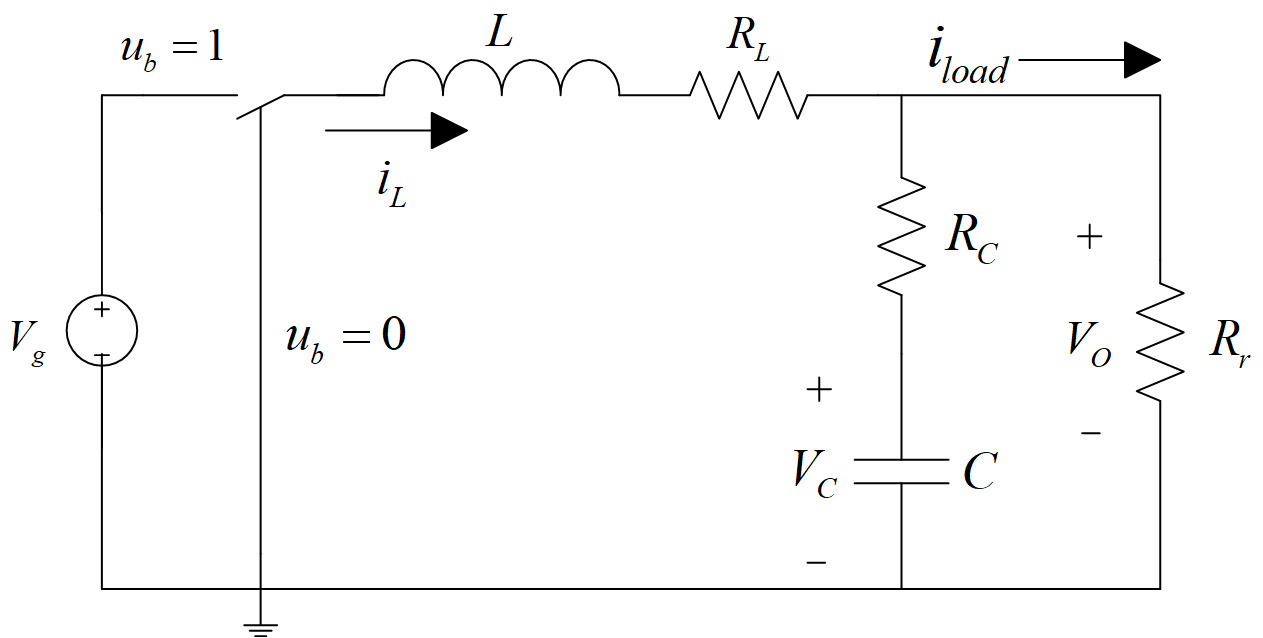
\includegraphics[width=3.5in]{picture/struck.jpg}\\
		\caption{Schematic of the buck converter.}\label{fig:schematic1}
	
\end{figure}

Mode 1: when $u_b=1$ which equals to the time zone $(0,dcT)$ of each switching period, it is easy to get the equations
\begin{equation}\label{onkvl}
\left\{ \begin{array}{l}
L\frac{{d{i_L}}}{{dt}} = {V_g} - {V_C} - {R_L} \cdot {i_L} - {R_C} \cdot C \cdot \frac{{d{V_C}}}{{dt}}\\
{V_C} + {R_C} \cdot C \cdot \frac{{d{V_C}}}{{dt}} = R_r \cdot \left( {{i_L} - C \cdot \frac{{d{V_C}}}{{dt}}} \right).
\end{array} \right.
\end{equation}

Leading to state-space formulation :
%\left[ {\begin{array}{*{20}{c}}
%	{ - \frac{1}{L} \cdot \frac{{R \cdot {R_C} + R \cdot {R_L} + {R_L} \cdot {R_C}}}{{R + {R_C}}}}&{ - \frac{1}{L} \cdot \frac{R}{{R + {R_C}}}}\\
%	{\frac{1}{C} \cdot \frac{R}{{R + {R_C}}}}&{\frac{1}{C} \cdot \frac{1}{{R + {R_C}}}}
%	\end{array}} \right]
\begin{equation}\label{onsol}
\left[ \begin{array}{l}
{{\dot i}_L}(t)\\
{{\dot V}_C}(t)
\end{array} \right] = A_{ss} \left[ \begin{array}{l}
{i_L}(t)\\
{V_C}(t)
\end{array} \right] + \left[ \begin{array}{l}
\frac{1}{L}\\
0
\end{array} \right]{V_g}.
\end{equation}
Here $A_{ss}=\left[ {\begin{array}{*{20}{c}}
	{ - \frac{1}{L} \cdot \frac{{R_r \cdot {R_C} + R_r \cdot {R_L} + {R_L} \cdot {R_C}}}{{R_r + {R_C}}}}&{ - \frac{1}{L} \cdot \frac{R_r}{{R_r + {R_C}}}}\\
	{\frac{1}{C} \cdot \frac{R_r}{{R_r + {R_C}}}}&{\frac{1}{C} \cdot \frac{1}{{R_r + {R_C}}}}
	\end{array}} \right]$,
${{\dot i}_L}(t)=\frac{{d{i_L}}}{{dt}}$ and ${{\dot V}_C}(t)=\frac{{d{V_C}}}{{dt}}$, similarly hereinafter.

Mode 2: when $u_b=0$ which equals to the time zone $(dcT,T)$ of each switching period, the equations can also be set up as follows:
\begin{equation}\label{kvloff}
\left\{ \begin{array}{l}
0 = L\frac{{d{i_L}}}{{dt}} + {R_L} \cdot {i_L} + {V_C} + C \cdot {R_C} \cdot \frac{{d{V_C}}}{{dt}}\\
{V_C} + C \cdot {R_C} \cdot \frac{{d{V_C}}}{{dt}} = R_r \cdot ({i_L} - \frac{1}{C} \cdot \frac{{d{V_C}}}{{dt}}).
\end{array} \right.
\end{equation}

Leading to the state-space formulation:
\begin{equation}\label{soloff}
\left[ \begin{array}{l}
{\dot {i}_L}(t)\\
{{\dot V}_C}(t)
\end{array} \right] =A_{ss}\left[ \begin{array}{l}
{i_L}(t)\\
{V_C}(t)
\end{array} \right].
\end{equation}

In fact, the equivalent series resistances of the capacitor and inductance are small enough to be neglected. Under this assumption, the matrices of the state-space functions in mode 1 (\ref{onsol}) and mode 2 (\ref{soloff}) can be simplified as follows:
\begin{equation}\label{onmat}
{A_1} = \left[ {\begin{array}{*{20}{c}}
	0&{ - \frac{1}{L}}\\
	{\frac{1}{C}}&{ - \frac{1}{{R_r C}}}
	\end{array}} \right],{B_1} = \left[ {\begin{array}{*{20}{c}}
	{\frac{V_g}{L}}\\
	0
	\end{array}} \right]
\end{equation}

\begin{equation}\label{offmat}
{A_2} = \left[ {\begin{array}{*{20}{c}}
	0&{ - \frac{1}{L}}\\
	{\frac{1}{C}}&{ - \frac{1}{{R_r C}}}
	\end{array}} \right],{B_2} = \left[ {\begin{array}{*{20}{c}}
	0\\
	0
	\end{array}} \right].
\end{equation}

The following expression shows the state-space averaged model of a PWM converter \cite{leyva2006passivity}:
\begin{equation}\label{modelpwm}
\dot { x}(t) = A x(t) + {B_u} u(t),
\end{equation}
where
\begin{equation}\label{modelpara}
A = \left[ {\begin{array}{*{20}{c}}
	0&{ - \frac{1}{L}}\\
	{\frac{1}{C}}&{ - \frac{1}{{R_r C}}}
	\end{array}} \right],{B_u} = \left[ {\begin{array}{*{20}{c}}
	{\frac{{{V_g}}}{L}}\\
	0
	\end{array}} \right].
\end{equation}
and $x\left( t \right) = \left[ {\begin{array}{*{20}{c}}
	{{i_L}\left( t \right)}\\
	{{V_c}\left( t \right)}
	\end{array}} \right]$, $u(t)$ means the current duty-cycle $dc$ as the PWM signal.

The matrices $A$, $B_u$ in (\ref{modelpara}) may be uncertain and time varying. Especially $B_u$ depends on input voltage $V_g$, which leads to the LPV model \cite{sadek2016fpga} and is described as follows:
\begin{equation}\label{modelpwmlpv}
\dot { x}(t) = A(t) x(t) + {B_u}(t) u(t),
\end{equation}
where
\begin{equation}\label{modelparalpv}
A(t) = \left[ {\begin{array}{*{20}{c}}
	0&{ - \frac{1}{L}}\\
	{\frac{1}{C}}&{ - \frac{1}{{R_r(t)C}}}
	\end{array}} \right],{B_u}(t) = \left[ {\begin{array}{*{20}{c}}
	{\frac{{{V_g}(t)}}{L}}\\
	0
	\end{array}} \right].
\end{equation}
This LPV model will be used in Section \ref{sec:CPM} to design an MPC controller for the buck DC-DC converter.

\section{Numerical Simulations and Experiments Certificate} \label{sec:Numerical}

Now the performance of the algorithm proposed in Section \ref{sec:CPM} will be tested for the problem described in Section \ref{sec:FDR}. As the tracking target is the output voltage but not the state, the first thing is to get the working point $(x_{ref},u_{ref})$ mentioned in (\ref{costf}) by solving the linear system coming from the model (\ref{modelpwm})

\begin{subequations}
	\begin{numcases}{}
	{{x_{ref}} = A{x_{ref}} + {B_u}{u_{ref}}}\\
	{{y_{ref}} = C_m {x_{ref}}}\label{outputc}
	\end{numcases}
\end{subequations}
at each sampling time, leading to the linear function
\begin{equation}\label{linearfun}
\left[ \begin{array}{l}
{x_{ref}}\\
{u_{ref}}
\end{array} \right] = {\left[ {\begin{array}{*{20}{c}}
		{{I_{{n_x}}}}&{ - B}\\
		C_m &0
		\end{array}} \right]^{ - 1}}\left[ {\begin{array}{*{20}{c}}
	0\\
	{{y_{ref}}}
	\end{array}} \right].
\end{equation}

The output voltage $V_o$ (see Figure 1)
\begin{equation}\label{solvec}
{V_o} = C_m  \left[ {\begin{array}{*{20}{c}}
	{{i_L}\left( t \right)}\\
	{{V_C}\left( t \right)}
	\end{array}} \right],C_m = \left[ {\begin{array}{*{20}{c}}
	{\frac{{R_r \cdot {R_C}}}{{R_r + {R_C}}}}&{\frac{R_r}{{R_r + {R_C}}}}
	\end{array}} \right]
\end{equation}
equals to the output reference $y_{ref}$.

The numerical simulation study is carried out on a personal computer with the following configuration: Intel Core i7-2600 3.40GHz CPU, 4.00GB RAM, 64-bit Windows 10 Operating System. The model is implemented in PLECS and the experiments are based on NI CompactRIO platform using Xilinx FPGA.



\subsection{Numerical Simulations}\label{subsec}

The values of the converter parameters set are shown in Table \ref{tabparam}. The nominal value of the supply voltage is 5 V. Sampling time ${T_s} = 0.01ms$ is set to form the discrete model (\ref{mpcmodel}): $x_k \in \mathbb{R}^2$, $u_k\in \mathbb{R}$, $A = \left[ {\begin{array}{*{20}{c}}
	{0.9672}&{ - 0.2992}\\
	{0.0224}&{0.9983}
	\end{array}} \right], C_m = \left[ {\begin{array}{*{20}{c}}
	{0.0269}&{0.9980}
	\end{array}} \right]$. As the experiments are made on a fixed resistive load, $A(t)$ in (\ref{modelparalpv}) is a fixed one while ${B_u}$ changes with the sawtooth input voltage at each sampling time. For MPC, the weights $Q = \left[ {\begin{array}{*{20}{c}}
	1&0\\
	0&1
	\end{array}} \right], R=800$ is a trial in the cost function. The constraints come from the real limit of the duty-cycle ranging from 0 to 1. The predictive horizon $N$ is set to 10.

\begin{table}[h]
	\caption{Buck DC-DC Converter Parameters}\label{tabparam}
	\begin{center}
		\begin{tabular}{c|c }
			\hline
			\hline
			Parameter & Value  \\
			\hline
			$R_r$ & 10 $\Omega $ \\
			\hline
			$R_C$ & 0.027 $\Omega $\\
			\hline
			$L$ & 33 $\mu$ H\\
			\hline
			$C$& 440 $\mu$ F\\
			\hline
			$V_g$&[7 , 12] V\\
			\hline
			$V_o (V_{ref})$& 5 V\\
			\hline
			$T_s$ & 0.01 ms\\
			\hline
			\hline
		\end{tabular}
	\end{center}
\end{table}







The professional software PLECS is used to model and simulate the circuit in Figure \ref{fig:feedback}. Typical power electronics components such as semiconductors, inductors and capacitors are placed on the circuit diagram and simply connected by drawing wires \cite{alimeling1999plecs}. The parameters come from the real converters shown in Table \ref{tabparam} and the simulations are done to test whether the closed loop using the MPC controller proposed in this paper is fit for wind turbine generator. From \cite{middlebrook1976general} and \cite{middlebrook1977general}, it is known that in CCM mode, when the MOSFET works in high level which depends on the PWM signal, the diode will switch-off and when the MOSFET works in low level, the diode will be on. To model the converter easier, the two modes will be replaced by a switch just like the one in Figure \ref{fig:schematic1}. However, in Figure \ref{fig:feedback}, there are some more parameters such as resistances $r_{ds}$ and $r_d$ which can be neglected when modelling because their values are far more smaller than the resistances $R_L$, $R_C$ and $R_r$. Meanwhile, $R_{up}$ and $R_{down}$ are divider resistances used for protecting the circuit from high voltage and current. And these two resistances will not influence the modelling of the converter as in the digital control $V_{fb}$ will be transferred to $V_o$ by ${V_{fb}} = \frac{{{R_{down}}}}{{{R_{up}} + {R_{down}}}}{V_o}$ to compare with $V_{ref}$.

\begin{figure}
	\begin{center}
		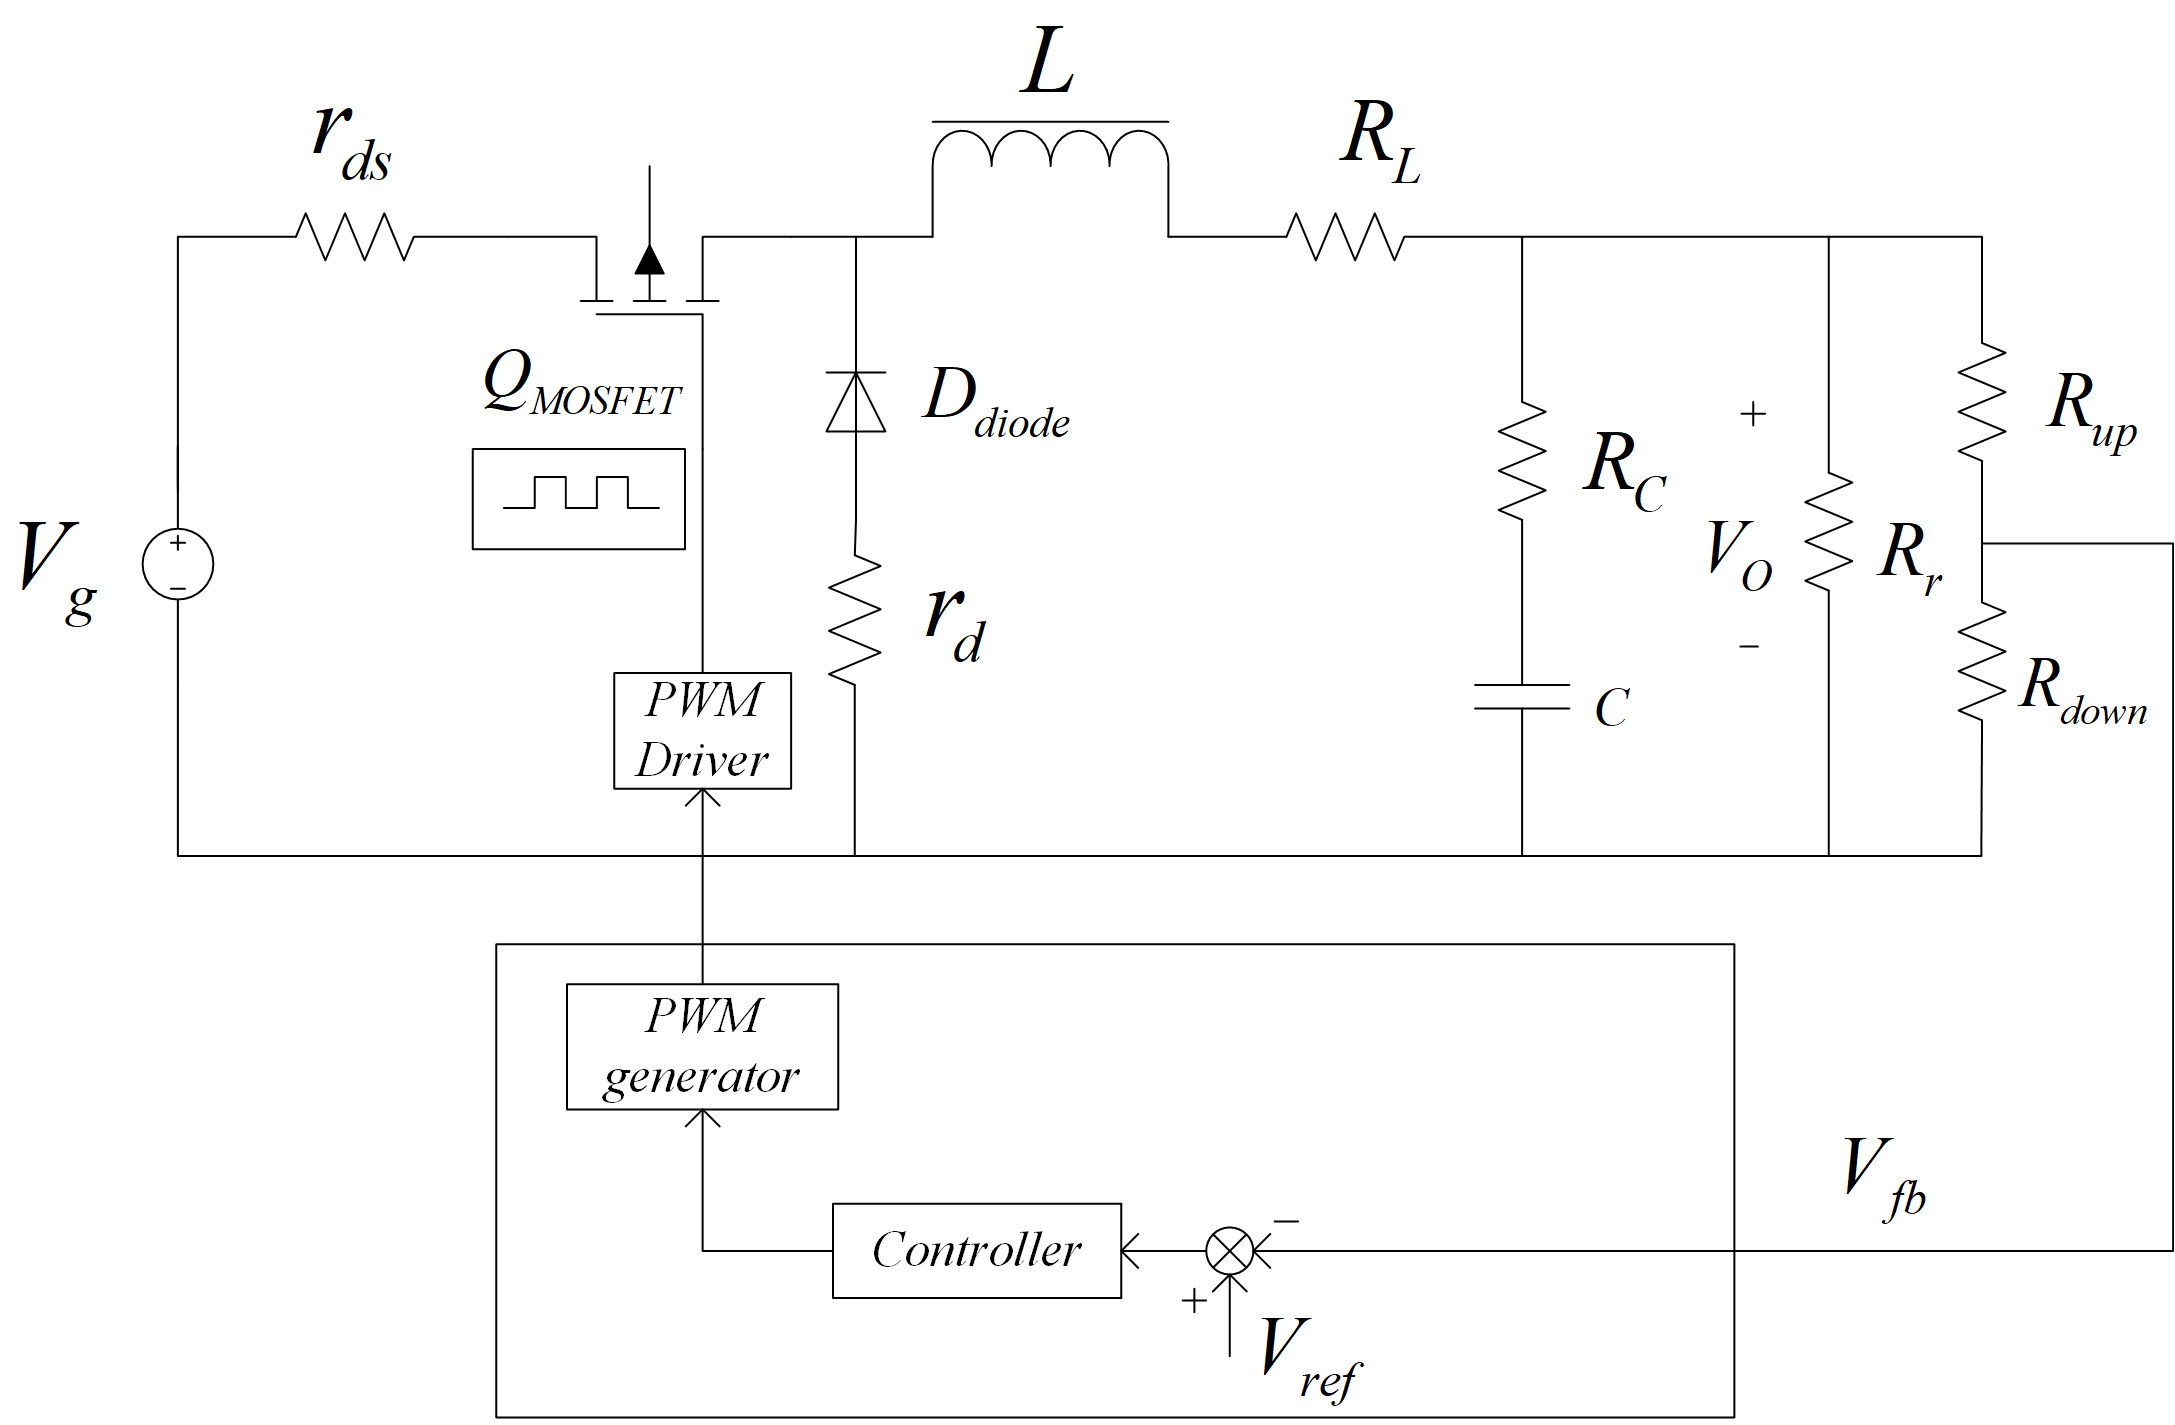
\includegraphics[width=3.5in]{picture/str.jpg}
		\caption{Control design of buck converter in PLECS.}\label{fig:feedback}
	\end{center}
\end{figure}

First before implementing the MPC controller to the real-time platform, a comparison is made between the PID controller and the MPC controller as DC-DC converter is an SISO LPV system with variable gain. Figure \ref{fig:pidmpcsi} shows a simulation between the PID controller and the MPC controller based on PLECS-Simulink.  The output set-point of the Buck DC-DC is set as 5V and the load is 10$\Omega$. Figure \ref{fig:1} depicts that MPC can provide a smaller overshoot and a faster converging time than the PID controller. What is more in the figure, if the inductor current is imited to $\left[ 0,15\rm {A} \right]$, in contrast to MPC, the PID controller cannot satisfy the state constraints since the PID controller only works on the input-output constraints \cite{afram2014theory}.
\begin{figure*}
	\centering
	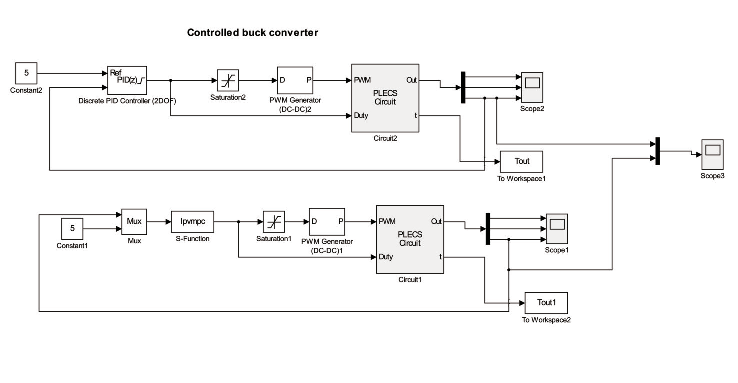
\includegraphics[width=7in]{picture/lz123.pdf}\\
	\caption{Simulation comparison between PID and MPC controllers through PLECS Simulation.}\label{fig:pidmpcsi}
\end{figure*}
\begin{figure*}\centering
	\subfigure[Inductor current of the process using MPC and PID controller.] {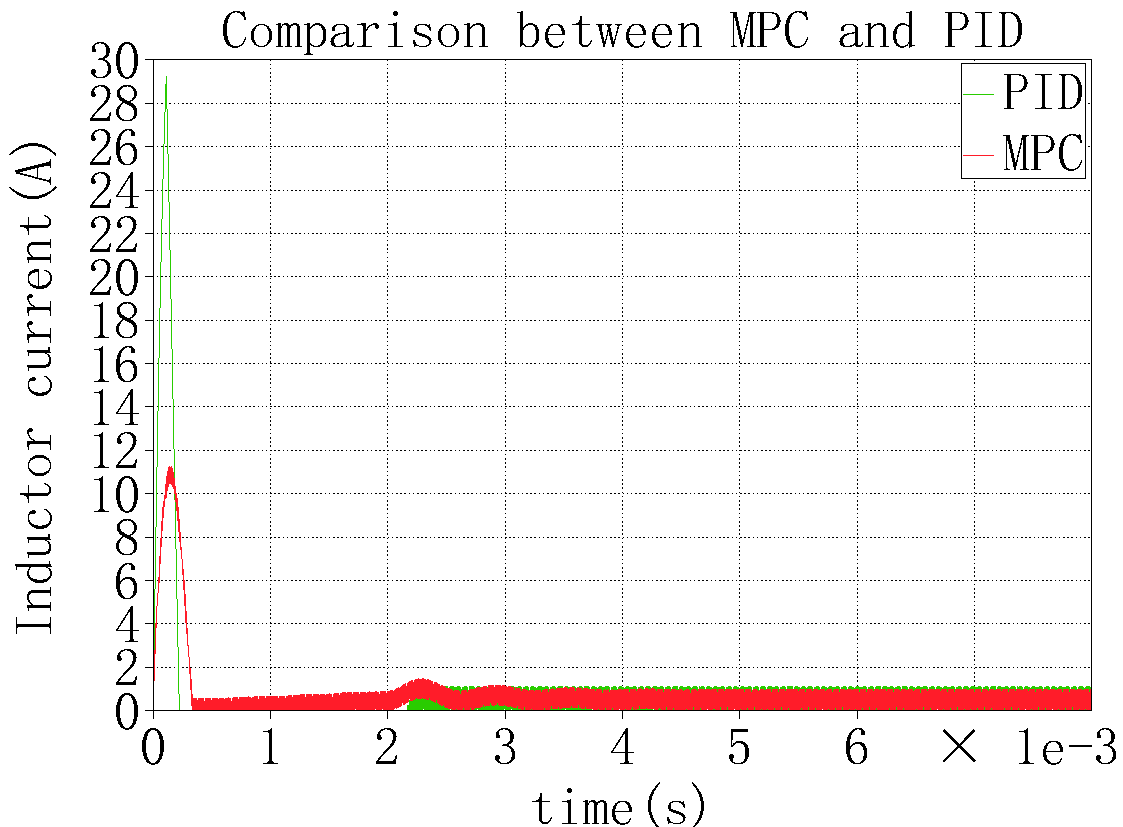
\includegraphics[width=0.45\textwidth]{picture/scope.pdf}}
	\hspace{0.5in}
	\subfigure[Output voltage of the process using MPC and PID controller.] {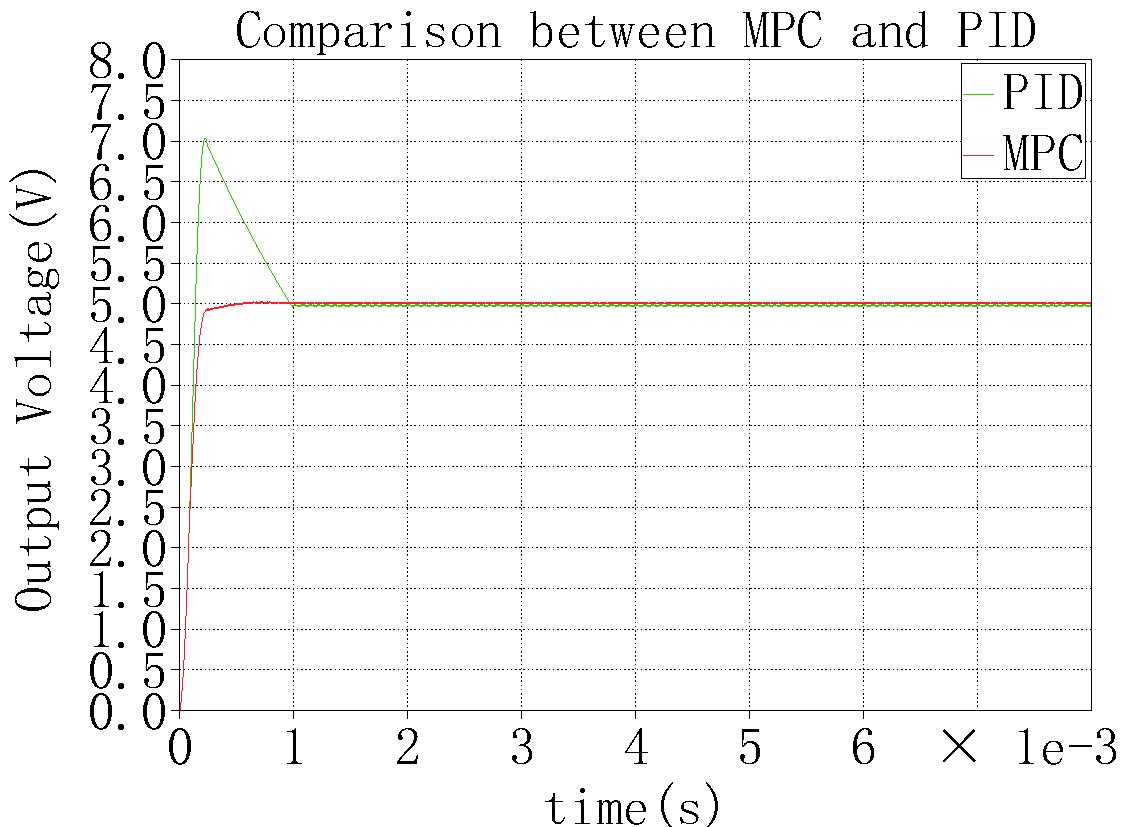
\includegraphics[width=0.45\textwidth]{picture/scopeoutput.pdf}}
	\caption{Simulation curves between PID and MPC controllers. }
	\label{fig:1}
\end{figure*}

Figure \ref{fig:plecsclose} shows the simulation of the buck converter working in closed loop with sawtooth input voltages which is similar to the real process. The buck DC-DC converter acts as a second-order asymptotically stable system, although a ripple wave resists in steady-state which will be demonstrated in the next experiments. Considering the modelling of the converter from Section \ref{sec:FDR}, regardless the noise from the environment, the main disturbance comes from the input voltage and the load. Figure \ref{fig:plecsclose} shows that no matter how the input voltages change, the closed loop system using the proposed MPC algorithm can reach a desired output voltage and this controller will be implemented in real-time platform in the next section.
\begin{figure*}\centering
	\subfigure[The whole process executed similar to the real process.] {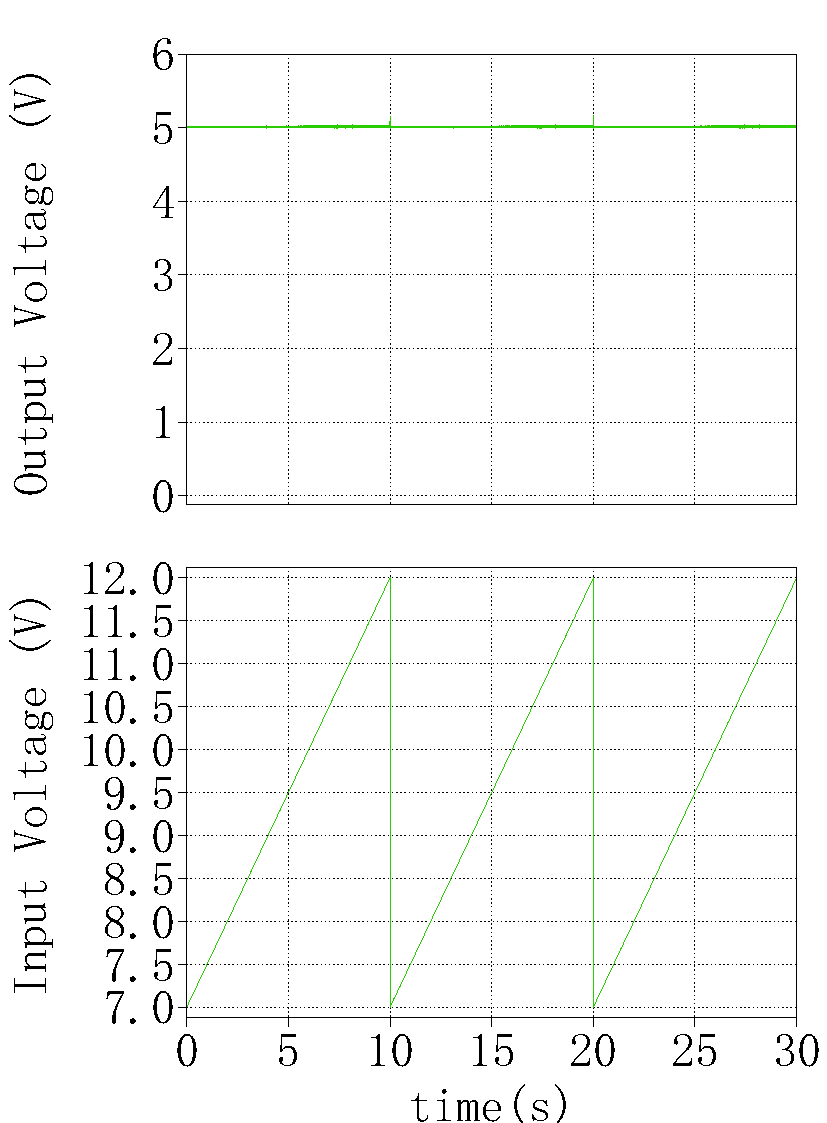
\includegraphics[width=0.45\textwidth]{picture/scope31.pdf}}
	\hspace{0.5in}
	\subfigure[The starting curve in the first second of the process.] {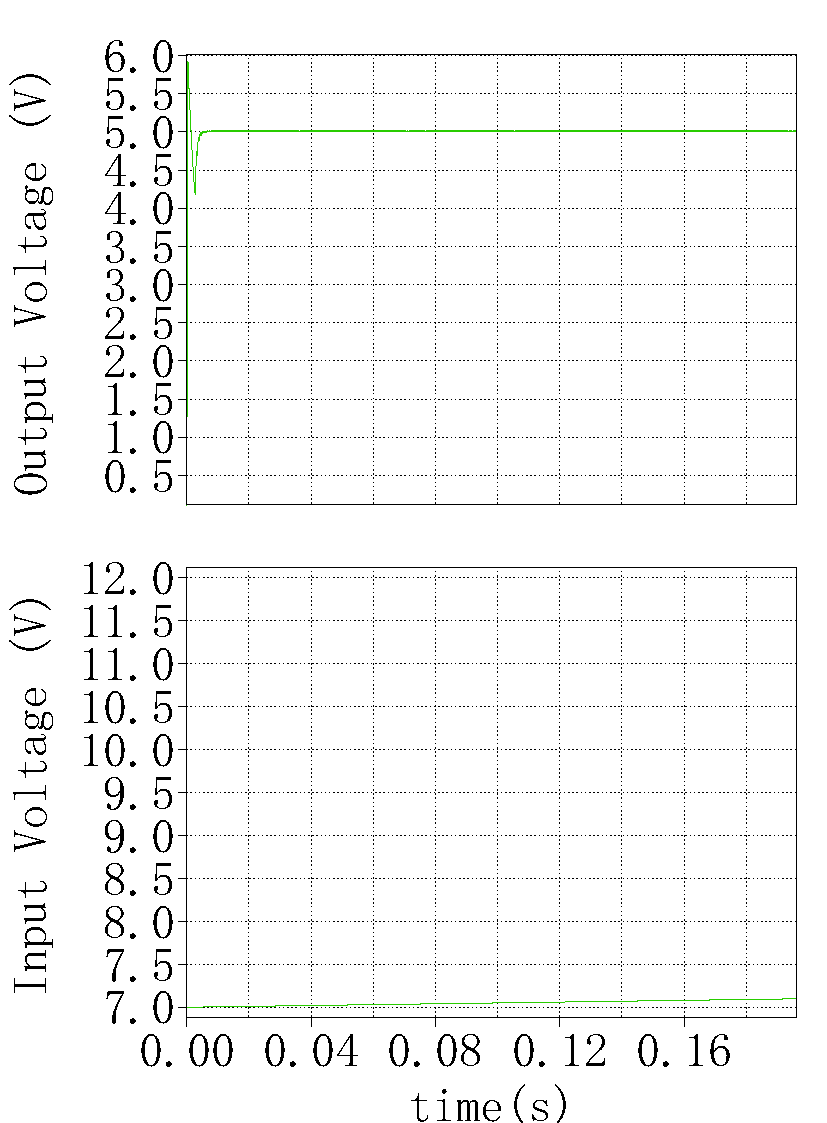
\includegraphics[width=0.45\textwidth]{picture/scope10.pdf}}
	\caption{Closed loop with a sawtooth input voltage. }
	\label{fig:plecsclose}
\end{figure*}

\subsection{Comparison with existing approaches}

The numerical simulation comparisons between the algorithm proposed in this paper and the other state-of-art QP solvers are running on PC: Intel Core i7-2600 3.40GHz CPU, 4.00GB RAM, 64-bit Windows 10 Operating System and MATLAB R2016a. All the solvers share the same model and its coefficient parameters containing discrete model parameter $A$, $C_m$, the weights $Q$, $R$, set-point and the constrains in the last section. Meanwhile the discrete matrix $B_u$ changes with the sawtooth input voltage at each sampling time and all the simulations follow the same rhythm when the model updates mentioned in Section \ref{subsec}. To compare the optimization performances of these algorithms, different prediction horizons have been used to form QP problems with different scales. Note that t he computational time of both formulating and solving QP problem is recorded.  More precisely, in each control step, the MPC problem is converted to QP and solved 50 times, and the minimum is recorded. Finally  the whole process is set in 100-control-step and the minimum time at each step is accumulated.
\begin{table*}[h]
	\centering
	\fontsize{7.5}{20}\selectfont
	\caption{The maximum and minimum iterations of the algorithms at different predictive horizons.}
	\label{tab:iteration}
	\begin{tabular}{|c|c|c|c|c|c|c|c|c|c|c|}
		\hline
		\multirow{2}{*}{Algorithms}&
		\multicolumn{2}{c|}{N=10}&\multicolumn{2}{c|}{N=15}&\multicolumn{2}{c|}{N=20}&\multicolumn{2}{c|}{N=25}&\multicolumn{2}{c|}{N=30}\cr\cline{2-11}
		&iter.(min)&iter.(max)&iter.(min)&iter.(max)&iter.(min)&iter.(max)&iter.(min)&iter.(max)&iter.(min)&iter.(max)\cr
		\hline
		\hline
		non-condensed PWA fmpc&1&4&1&5&1&5&1&6&1&6\cr\hline
		ADMM&3&1000&3&1000&3&1000&3&1000&3&1000\cr\hline
		qpOASES&2&12&6&16&11&20&16&26&21&35\cr\hline
		OSQP&25&75&50&100&75&100&75&100&100&150\cr\hline
		GPAD&1&17&1&23&1&26&1&31&1&37\cr\hline
		non-condensed GPAD&88&284&115&358&122&365&131&411&155&423\cr\hline
		Gurobi&7&11&7&11&7&11&7&12&8&12\cr\hline
		non-condensed Gurobi&9&13&9&13&11&14&11&14&12&14\cr\hline
		Interior&3&7&3&8&3&9&3&9&3&9\cr\hline
		non-condensed Interior&4&7&4&8&4&8&4&9&4&10\cr\hline
	\end{tabular}
\end{table*}
\paragraph{Runtime Comparison}{The solver proposed in Section \ref{sec:CPM} is compared with other state-of-art QP solvers in a LPV-MPC problem of which the prediction horizons are between 10 and 100 with increment 10. To avoid the interrupts coming from other systems the solution will be executed at each sample step 50 times and the minimum time will be accepted for the particular simulation time. In Algorithm 1, as in \cite{patrinos2011global} it shows that $\tau $ is chosen based on the examples and after some trials $\tau {\rm{ = }}\frac{1}{{{\rm{1}}{\rm{.01}}\left\| D \right\|}}$ leads to a faster convergence. In addition, $\alpha  = 0.01$ and $\varepsilon  = \zeta  = 1e - 9$ are the settings of the proposed algorithm. The QP solvers considered in the comparison are interior-point, that also involves both primal and dual variables but has favorable sparsity pattern for MPC problems \cite{wang2010fast}, ADMM \cite{boyd2011distributed} and its OSQP variant \cite{osqp-infeasibility}, the online active-set solver qpOASES \cite{ferreau2014qpoases}, GPAD \cite{patrinos2014accelerated} and Gurobi \cite{Gurobi-toolbox-web}. About the settings of these algorithm, max-iteration is set to 1000 and the terminal tolerance is set to $ 1e - 9 $.}

Figure \ref{fig:compare} depicts the non-condensed piecewise smooth Newton method with exact line search (non-condensed PWA fast MPC) proposed in this paper keeps in a low runtime especially in long prediction horizon. The time order here is mainly based on the CPU scale, thus the time-scale ``seconds" does not mean the real time consuming in the embedded platform but can show the trend of each algorithm's cost.  Several observations based on the results demonstrate the superiority of the proposed algorithm. Although it does not perform much better than qpOASES, OSQP, GPAD and interior, when the prediction horizon increases, the computation time of the other algorithms increases a lot while the proposed algorithm keeps in a low degree. What is more all through the figure, the algorithms using sparse structure performs well when computation dimension increases.  Thus the special dealing with the equality function in the proposed MPC algorithms makes it much more scalable to the LPV problem size.
\begin{figure}
	\centering
		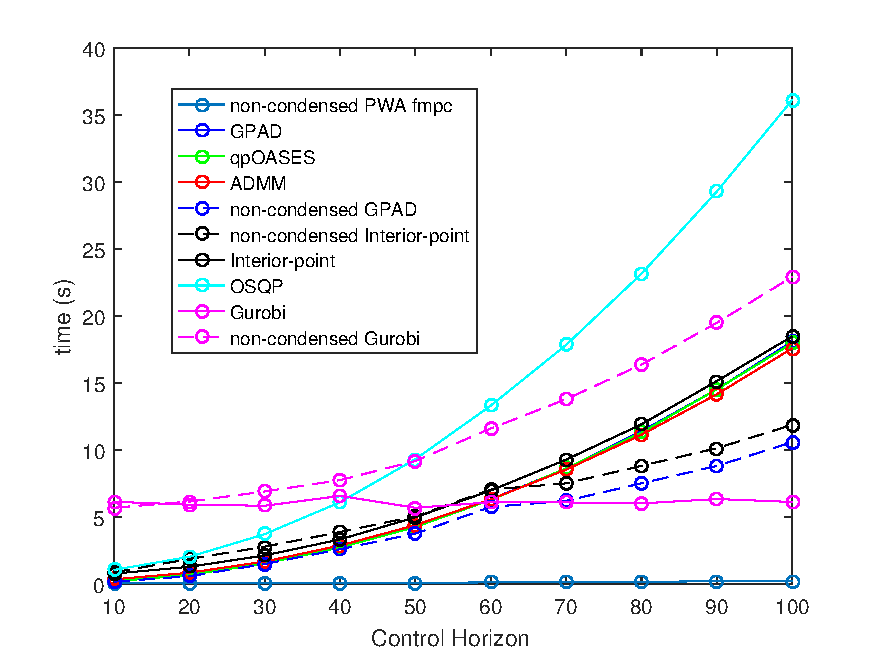
\includegraphics[width=3.5in]{picture/compare.pdf}
		\caption{Runtime with respect to prediction horizon comparison with existing approaches.}\label{fig:compare}
\end{figure}

\paragraph{Iterations Comparison}
The prediction horizon  will be set from 10 to 30 increased by 5 and the maximum as well as the minimum iterations of the benchmark solvers  are recorded during each sampling step. Table \ref{tab:iteration} depicts that the algorithm of this paper always keeps in a low number as the computation dimension augments while the others increase in some degree.


\begin{figure}
	\centering
	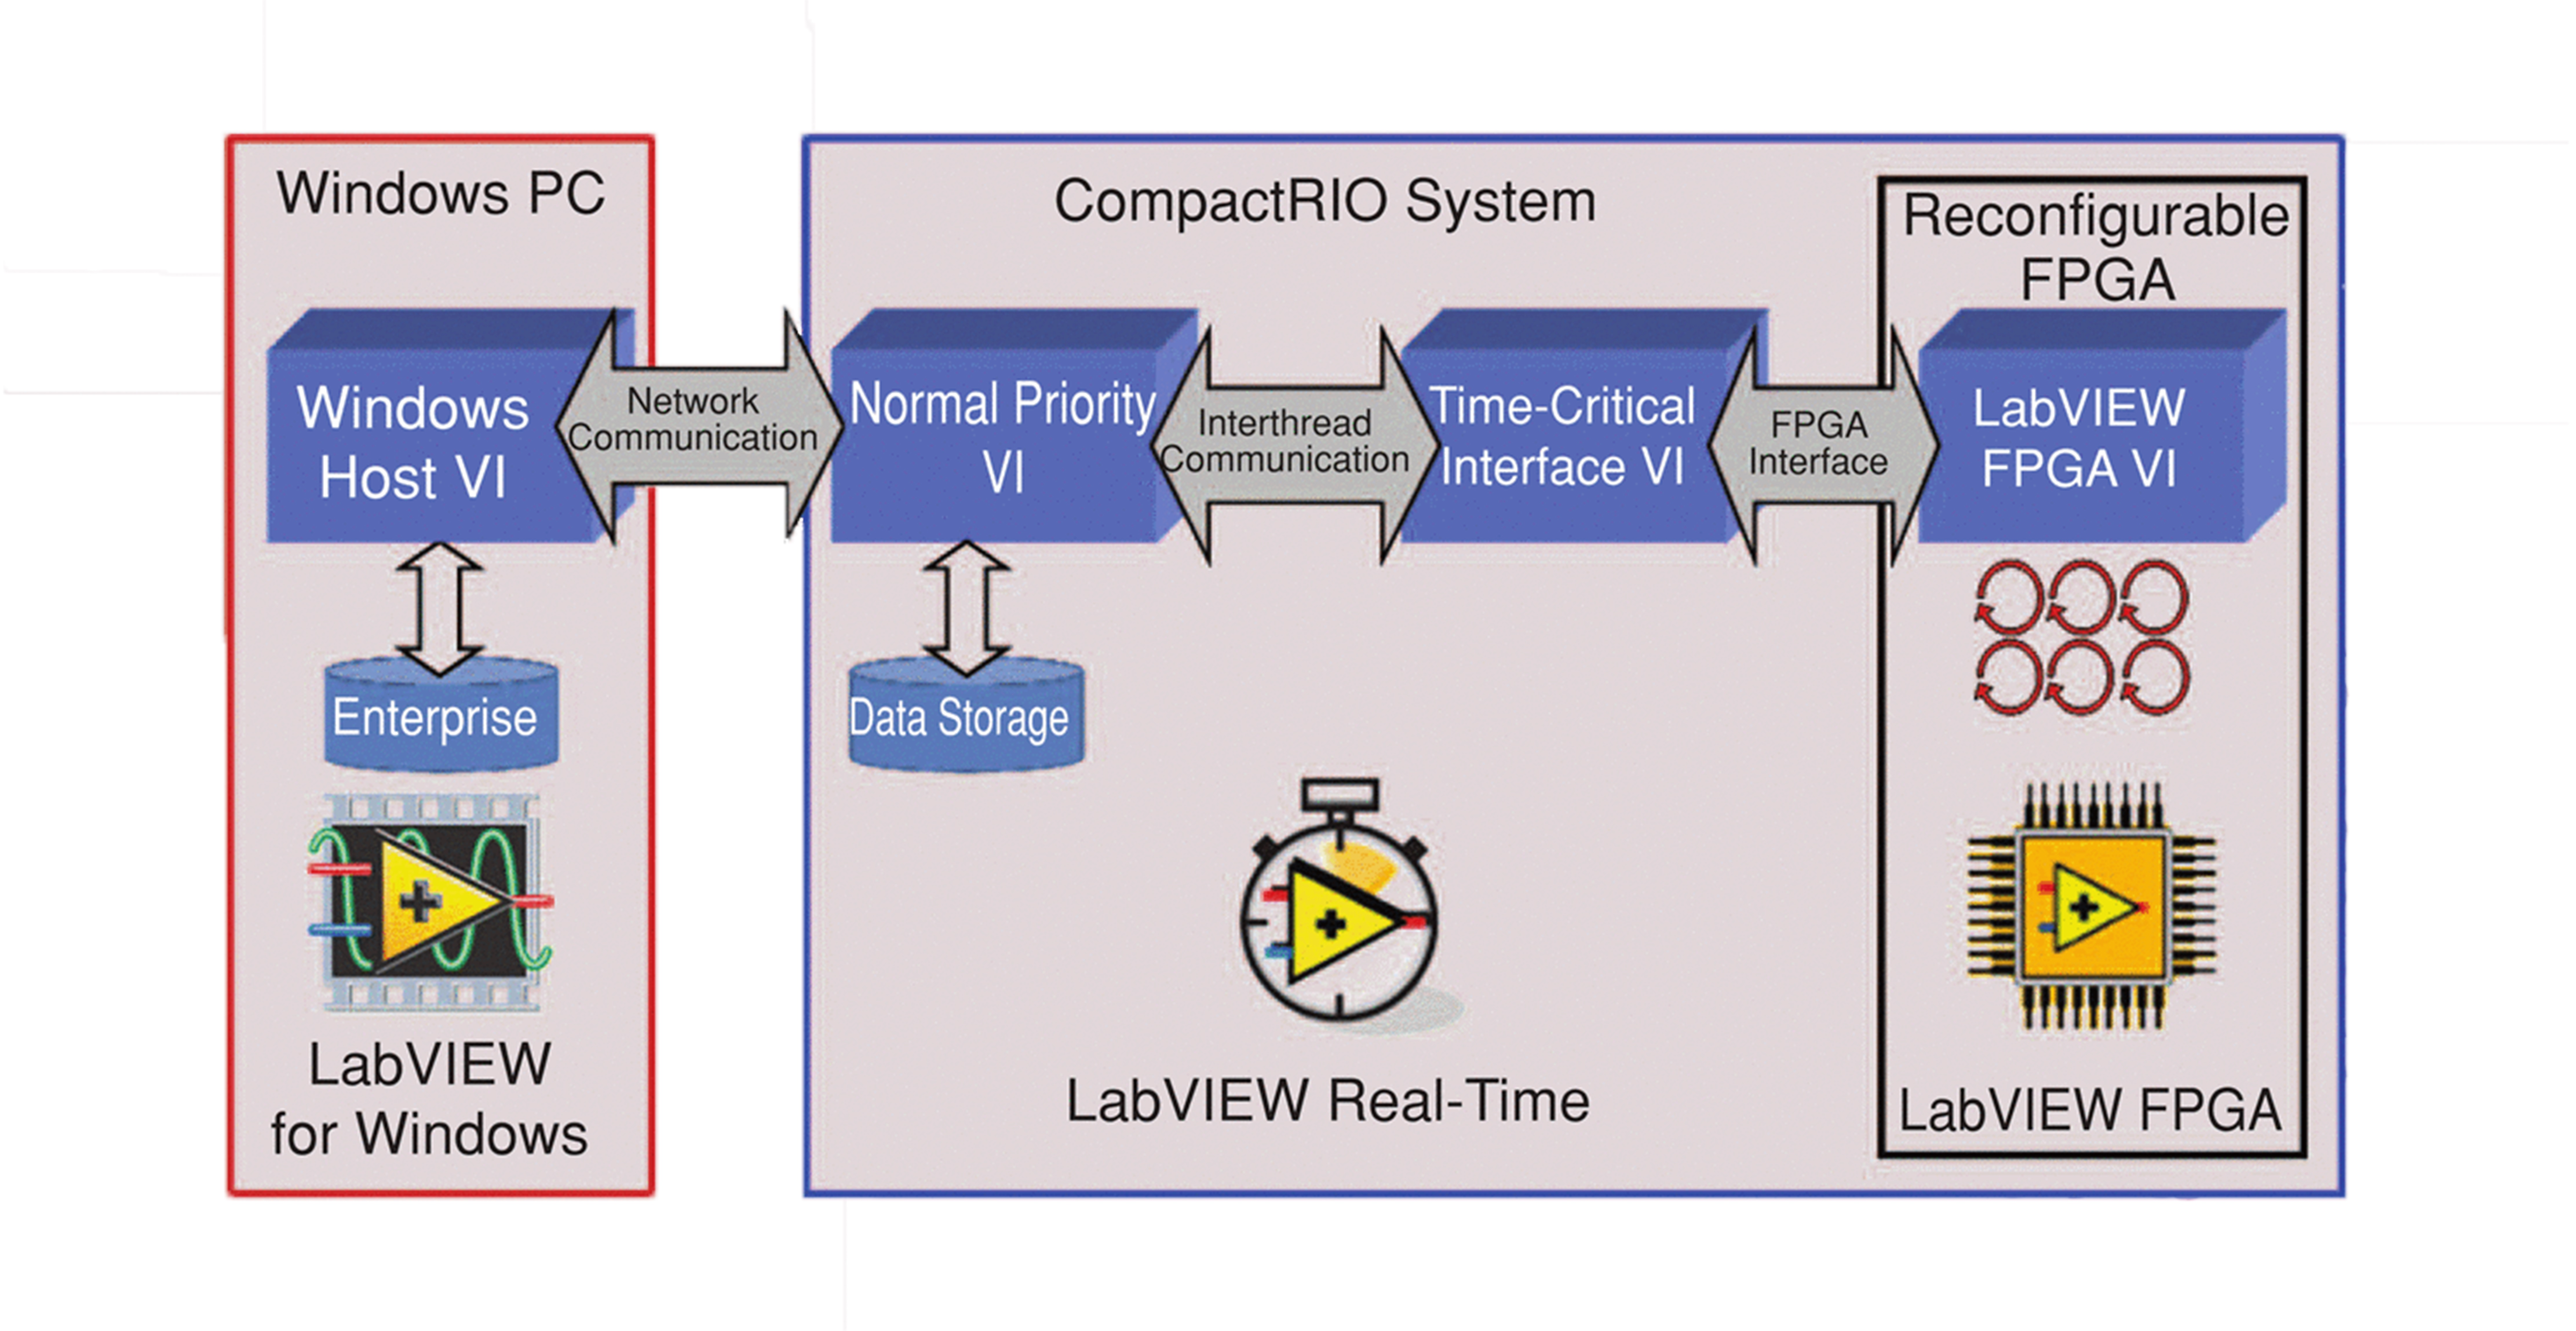
\includegraphics[width=0.45\textwidth]{picture/1.jpg}\\
	\caption{Software application architecture for NI CompactRIO platform.}\label{fig:clabview1}
\end{figure}

\subsection{Experiments}

Buck DC-DC converter is a typical switch-mode system and has an LPV model. Although existing control approaches have been proved effective, such as PID, sliding mode control and so on, several challenges have not been fully addressed yet, such as ease of controller design and tuning as well as robustness to load parameter variants \cite{quevedo2014predictive}. Moreover, PID control has its weakness in tuning and satisfying the state constraints compared with modern advanced control. Thus, the FPGA-experiments on Buck DC-DC converter are done on the platform National Instruments (NI) CompactRIO for verifying the algorithm whether efficient or not. The unique computational feature of this system is that it contains a real-time processor and an FPGA. Furthermore using the LABVIEW graphical development environment both devices are programmable. The CompactRIO platform uses cRIO-9082 with Xilinx FPGA (1.33 GHz, Dual Intel Core i7 CPU) as controller of which the time base is 40MHz and the precision reaches 100ppm (``ppm" stands for ``parts per million". It is like percent which is really parts per hundred but based on million instead of hundred. Therefore, 100ppm=100/1000000=0.01\%), cRIO-9223 as the 16-bit analog input ranging from -10V to 10V and maximum s ampling time 1M Samples/s and cRIO-9401 as the digital output (PWM) that has the feature of 8 channels, update rate 100ns and signal level 5V TTL (high level is 5V, low level is 0V). Figure \ref{fig:clabview1} is a software application architecture of the platform including a windows PC (host, monitoring and data storage), a real-time program (analog input sampling and digital output) running on the processor and an FPGA program (MPC implementation in IP builder), which contains several high-level blocks for control and signal processing that approximate floating-point implementation using the integer math available \cite{dase2006motorcycle}. The IP builder (shown in Figure \ref{fig:labv1}) mentioned before is to implement the MPC algorithm because it automatically optimizes the high level algorithm especially the matrix-vector multiplication, arrays and loops.

\begin{figure*}
	\begin{center}
		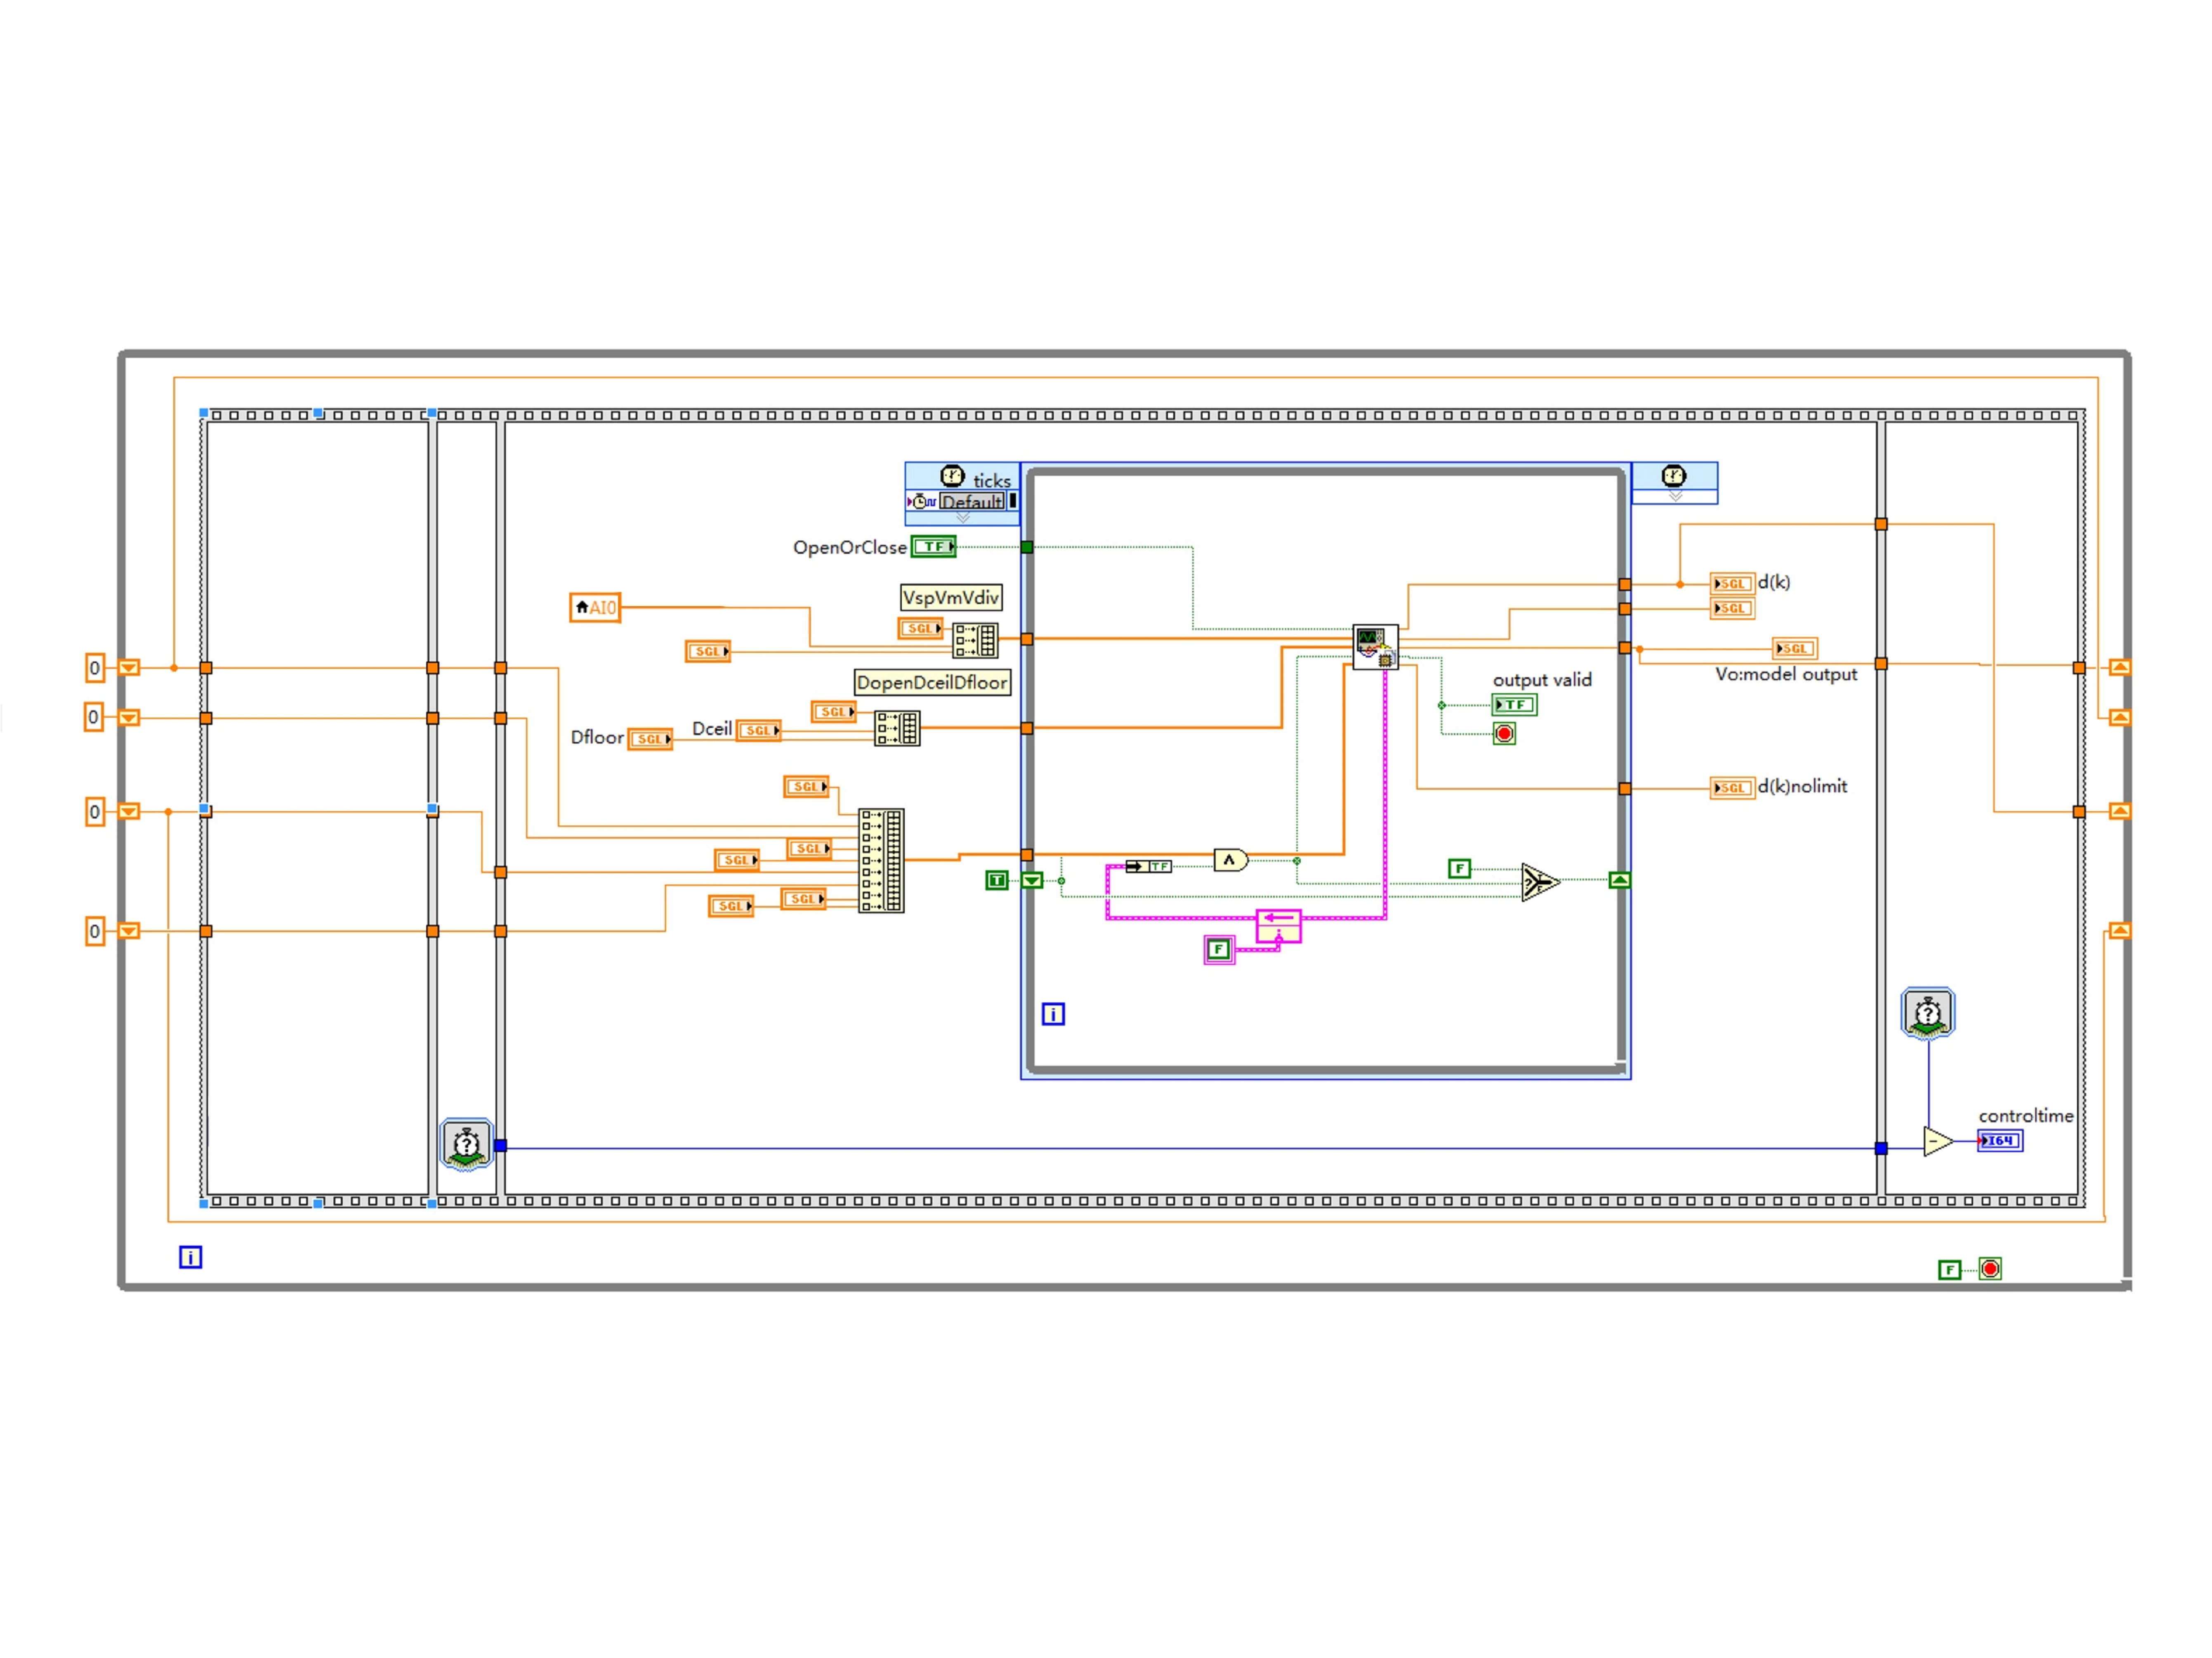
\includegraphics[width=5.5in]{picture/2.jpg}
		\caption{Implementing MPC using LABVIEW.}\label{fig:labv1}
	\end{center}
\end{figure*}

Although cRIO can run fast with high sampling frequency, it is still needed to prepare some divider resistances to satisfy the limitation of the I/O port. The Agilent DSO-X 3024A is chosen as the oscilloscope which has 4 channels with 200MHz width and the maximum sampling rate 4G Sample/s. To drive the converter, a 600W DC supply Agilent N6705B and a 500V/30A/750W DC load ITECH IT8813B are used as the resistance load. Finally a 100W wind generator NE-100S (which starts at a wind velocity 2m/s and stays stable at 10m/s) with a AC-DC converter is selected as the input of the system. When it  works around 3m/s inside the lab, the output DC voltage ranging from 7V to 12V. The whole structure of the platform is depicted in Figure \ref{fig:structure}.
\begin{figure*}
	\begin{center}
		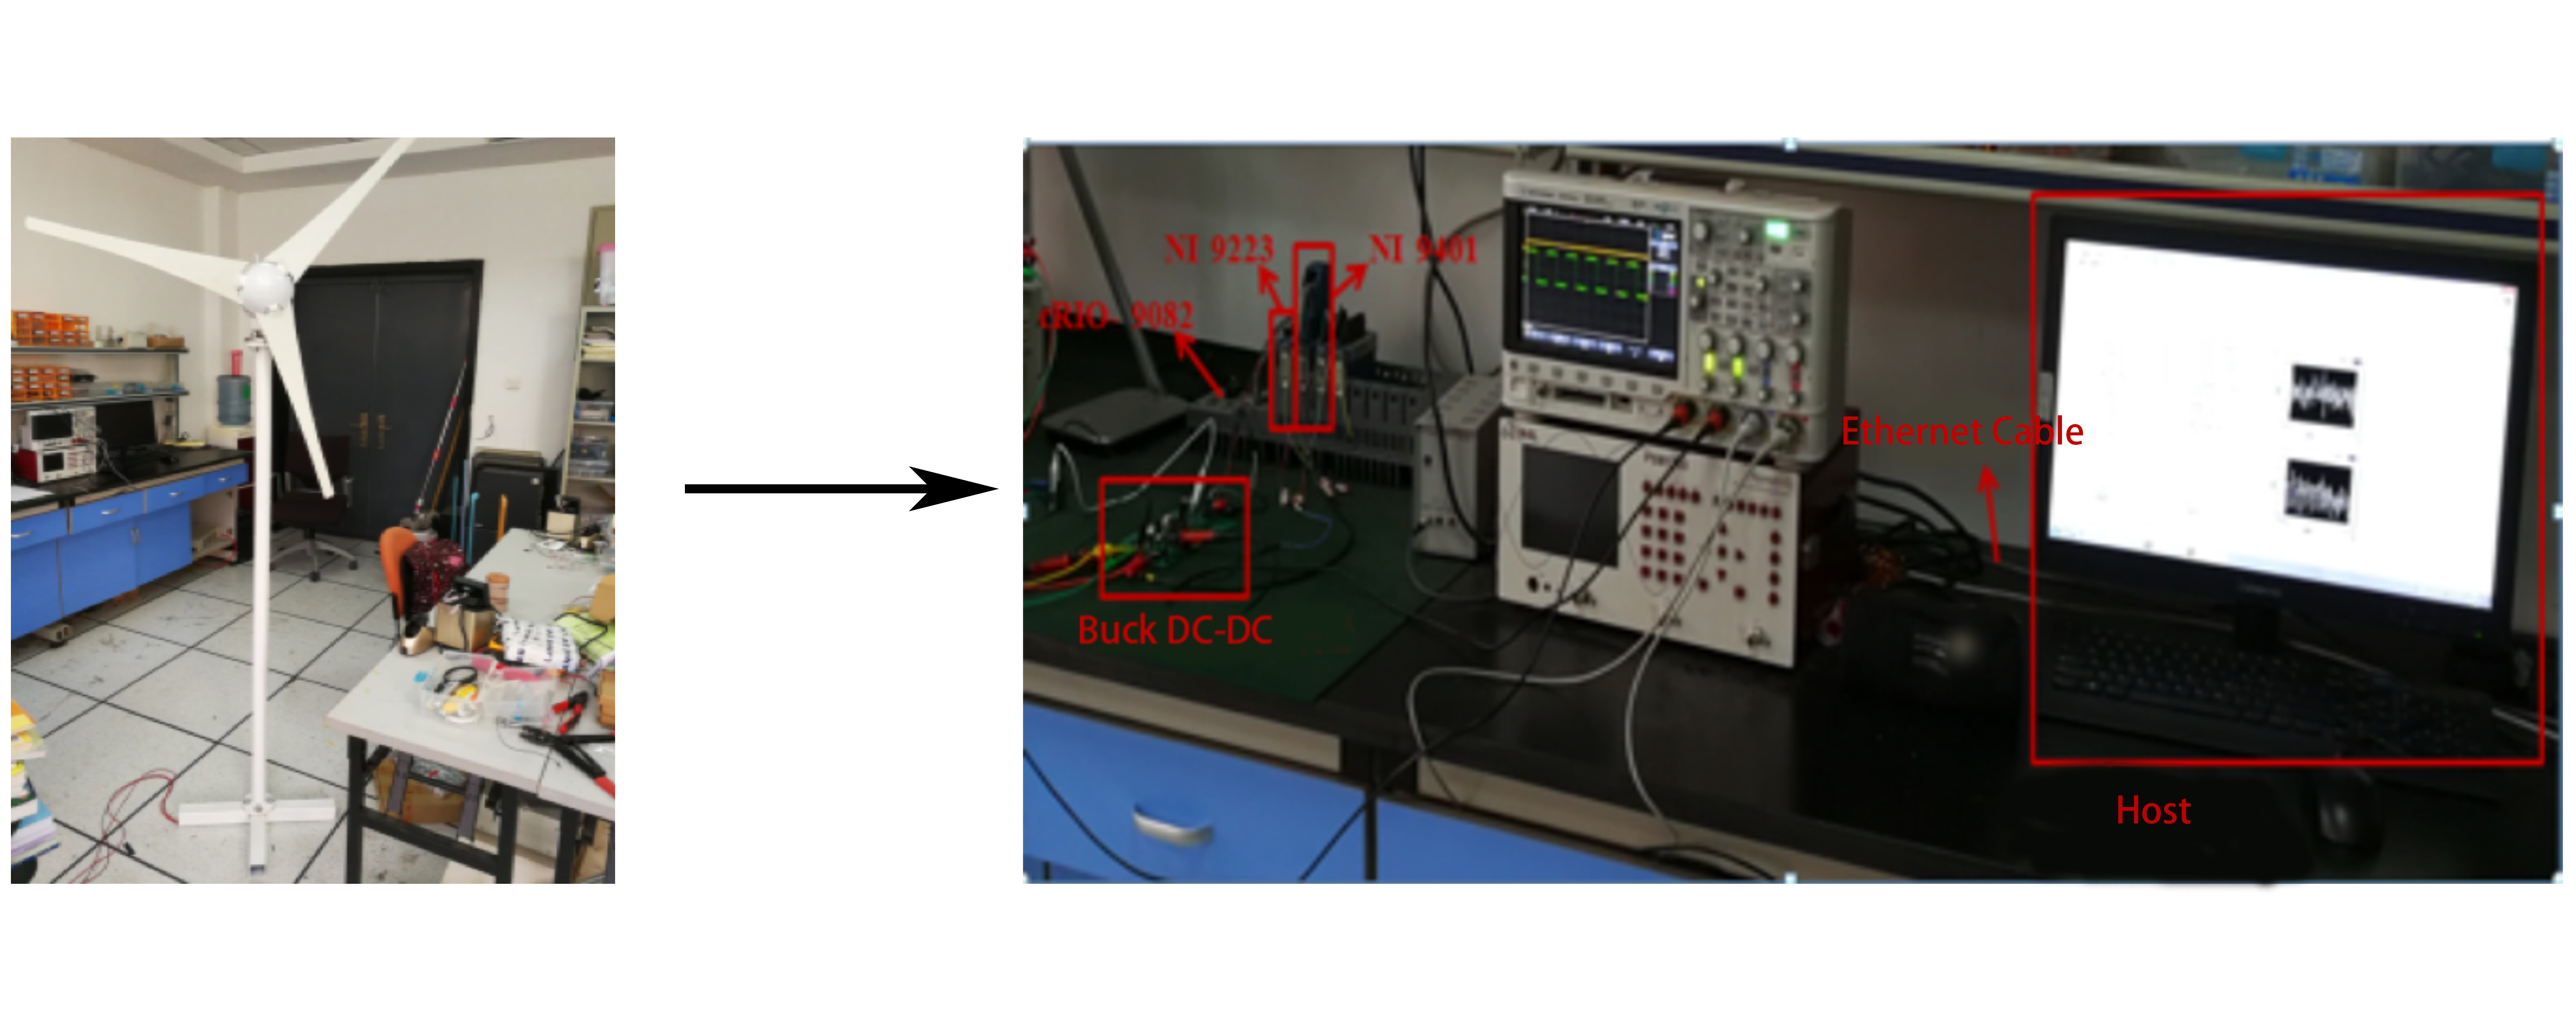
\includegraphics[width=5.5in]{picture/3.jpg}
		\caption{Experiment platform system setup.}\label{fig:structure}
	\end{center}
\end{figure*}

Both figures  in Figure \ref{fig:subfigosci} show that the wind turbine running in low-velocity generates a kind of sawtooth wave raging from 7V to 12V because the speed of the wind cannot reach the stable working point. In Figure \ref{fig:subfig1:a} it is shown that the system  changes much  around a certain output voltage with a large overshoot $ \pm 2.3$V taking no account of the ripple wave both in the input and the output generated by the converter itself. The upper curve in the figure is the input voltage as well as the lower one is output voltage. Both amplitudes of the voltage can be read in the picture (number 1 and 2 means two channels, the first is the input voltage and the second is output voltage) and the time scale is 2 seconds per grid. In Figure \ref{fig:subfig1:b} the overshoot is about $ \pm 0.7$V and neglecting the effect of the ripple wave, the output voltage has an average value of 4.95V  within  5$\%$ tolerable error. Thus the buck converter with the MPC controller can reach a desired output voltage and the overshoot in the process is less than that in the open loop system. Moreover, the MPC controller generates little overshoot when the input voltage changes in a sudden and it gets into the stable state faster than open loop.
\begin{figure*}
	\centering
	\subfigure[Open loop.] {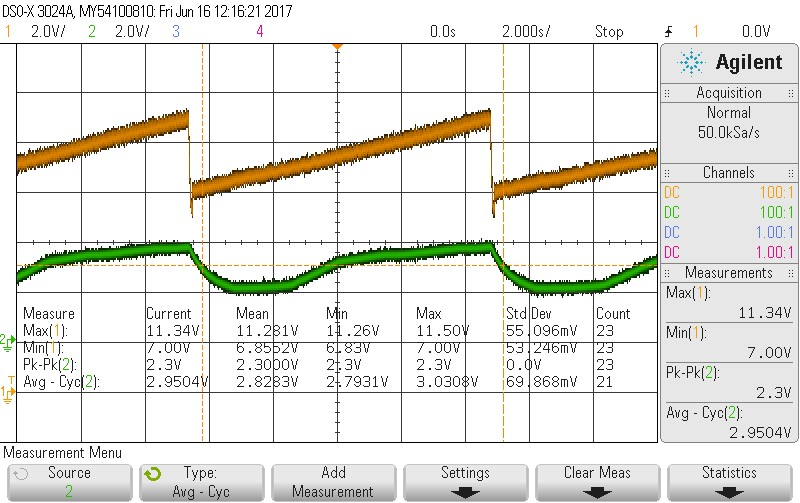
\includegraphics[width=0.40\textwidth]{picture/scopeopen.jpg}\label{fig:subfig1:a}}
	\hspace{0.5in}
	\subfigure[Closed loop.] {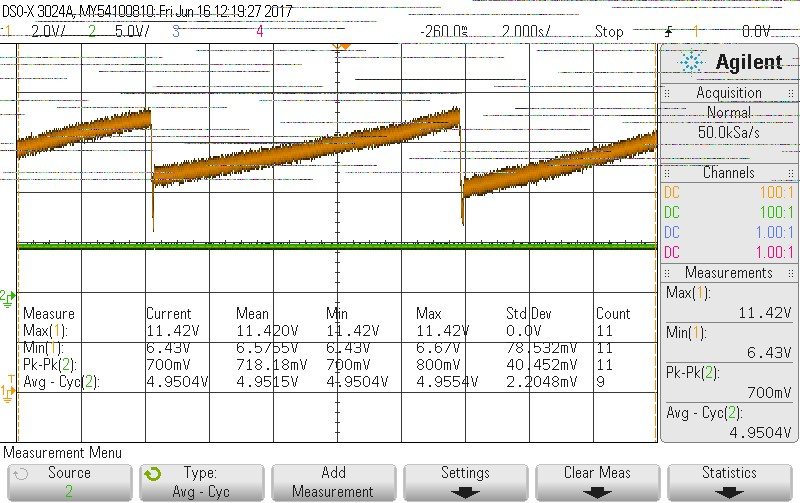
\includegraphics[width=0.40\textwidth]{picture/scopeclose.jpg}\label{fig:subfig1:b}}
	\caption{Oscilloscope image of input-output in the circuit. }
	\label{fig:subfigosci}
\end{figure*}

As the scope cannot save all the images to describe the whole process, the LABVIEW host provided by the cRIO will be used to observe a period of the process instead of a transient one. Figure \ref{fig:subfig} presents the sawtooth wave input and the output with fixed duty-cycle in open loop and MPC controller in closed loop system respectively. The LABVIEW host figure \ref{fig:subfig} records a history data after the system runs in 15 minutes (we choose only the first minute of the two states to show and compare) and x-axis of each picture depicts a period of time with the unit ``minute''. The system first works in an open-loop state and the output voltage violates with some oscillations shown in Figure \ref{fig:subfig:a}. Figure \ref{fig:subfig:b} shows  after several seconds in the 11th minute of the process, the system changes into close-loop state (the switch between open-loop and close-loop is operated online in the FPGA-host) and the output voltage converges and stays at a certain value 5V.
\begin{figure*}
	\centering
	\subfigure[Open loop.] {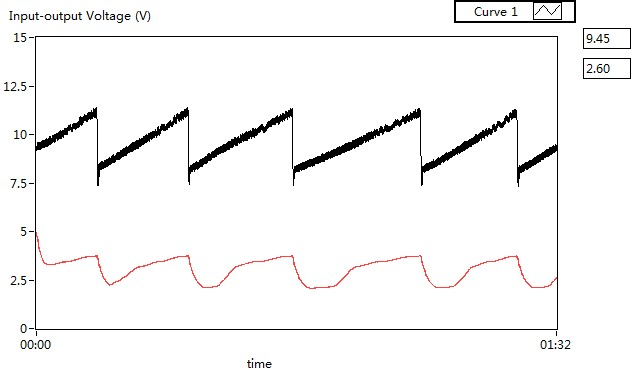
\includegraphics[width=0.45\textwidth]{picture/labviewb.jpg}\label{fig:subfig:a}}
	\hspace{0.5in}
	\subfigure[Close loop.] {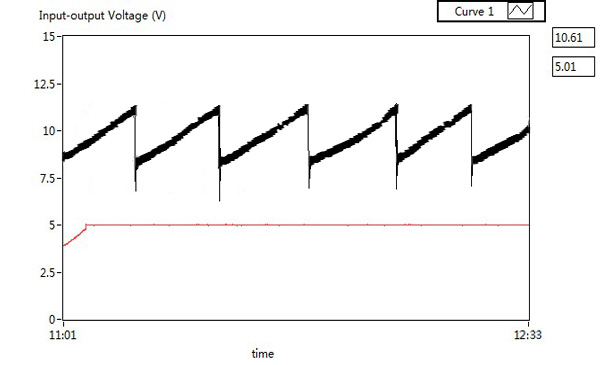
\includegraphics[width=0.45\textwidth]{picture/labview2.jpg}\label{fig:subfig:b}}
	\caption{Labview images of input-output voltage. }
	\label{fig:subfig}
\end{figure*}

\section{CONCLUSION} \label{sec:conclusion}

An effective computational method for linear parameter varying MPC and its application to buck converters is proposed and successfully tested in numerical simulations and FPGA platform experiments in this paper. The method mainly bases on a piecewise smooth Newton method with an exact line search used to solve a non-condensed QP formulation. As shown in this paper, this non-condensed MPC problem can be reformed to a non-condensed QP problem easily with no matrix-multiplication and most coefficient matrices are sparse as well as block triangular or diagonal which make the inverse during the optimization cost cheap. Meanwhile, the PWA equations for solving the QP problem require a low number of iterations, resulting in low CPU runtime when implementing the Newton method with exact line search because of the convergence properties \cite{chen1998newton}. Moreover the performance of the methodology shows well not only in comparison with several other algorithms though numerical test but also in a professional software simulation. Finally it is worth pointing out that this algorithm is implemented in the FPGA device to control the low velocity wind generator in the lab and shows its good response for the voltage's sudden break. In future research this algorithm will be tried in some other large-scale systems such as fluid transmission process \cite{ren2016dynamic,ren2018dynamic} which needs to track the multi-variables, UAV (unmanned aerial vehicle) to solve the problem composed by pitch angle, altitude, elevator angle with constraints \cite{ling2008embedded} and some other systems benefitting from the long horizon of MPC such as drivers with LC filters \cite{geyer2014benefit}, grid-connected converters \cite{lim2017long} and some other high power converters \cite{geyer2017model}, because of its fast runtime property in long prediction horizons and the good performance.

%\section{ACKNOWLEDGMENT}
%The authors wish to thank financial support from National Natural Science Foundation of P.R. China under grant No. 61134007, No. 61374121, and  the 111 Project under grant No. B07031.

\bibliographystyle{IEEEtran}
\bibliography{Zhen-Access}

% biography section
%
% If you have an EPS/PDF photo (graphicx package needed) extra braces are
% needed around the contents of the optional argument to biography to prevent
% the LaTeX parser from getting confused when it sees the complicated
% \includegraphics command within an optional argument. (You could create
% your own custom macro containing the \includegraphics command to make things
% simpler here.)
%\begin{IEEEbiography}[{\includegraphics[width=1in,height=1.25in,clip,keepaspectratio]{mshell}}]{Michael Shell}
% or if you just want to reserve a space for a photo:
\begin{IEEEbiography}[{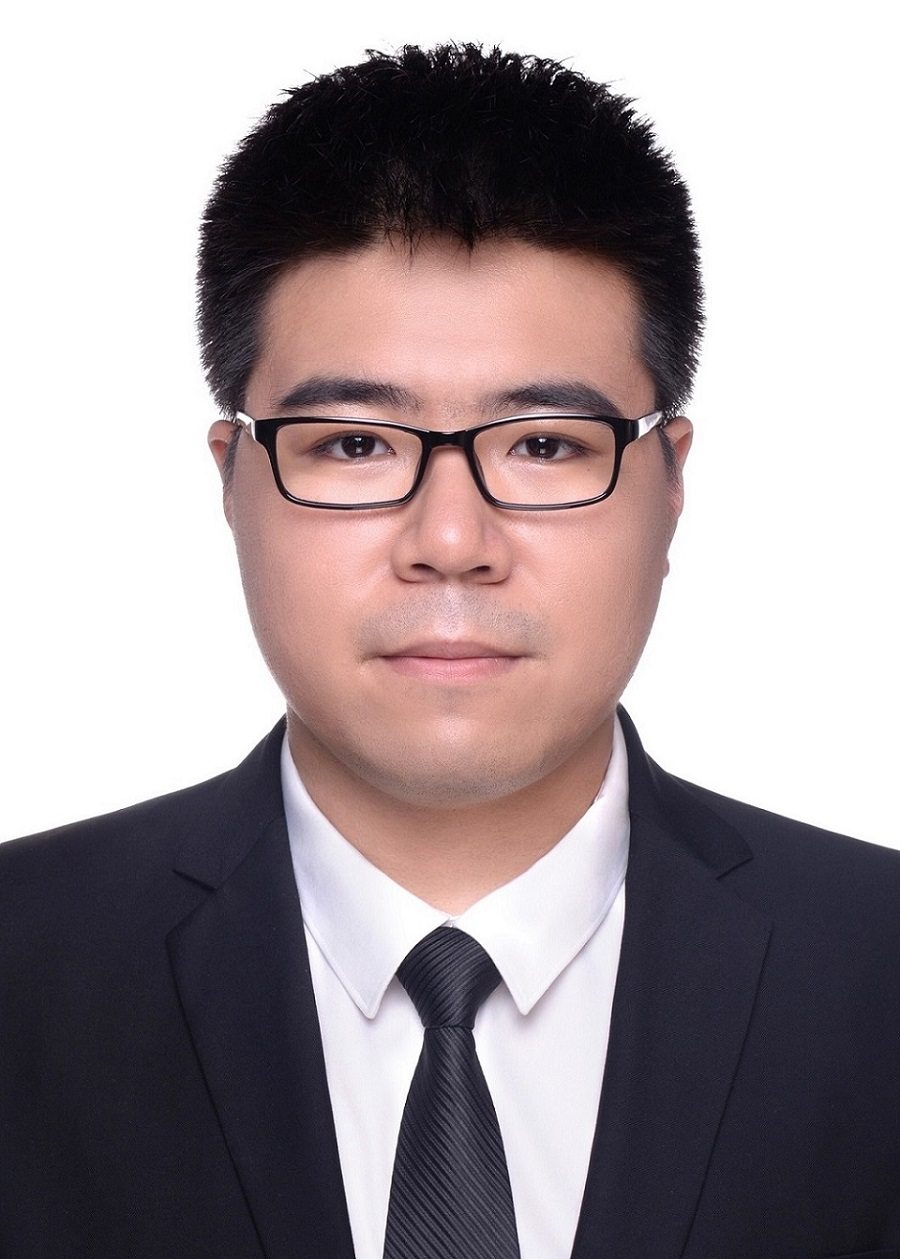
\includegraphics[width=1in,height
=1.25in,keepaspectratio]{Zhen_Liu}}]{Zhen Liu}
received his bachelor's degree in electrical engineering and automation from Zhejiang University, Hangzhou, China, in 2009, and Ph.D. degree in control science and engineering from Zhejiang University, Hangzhou, China, in 2018. His research interests include model predictive control, numerical simulation, optimal control theory and applications on embedded platform in power electronic.
\end{IEEEbiography}
\begin{IEEEbiography}[{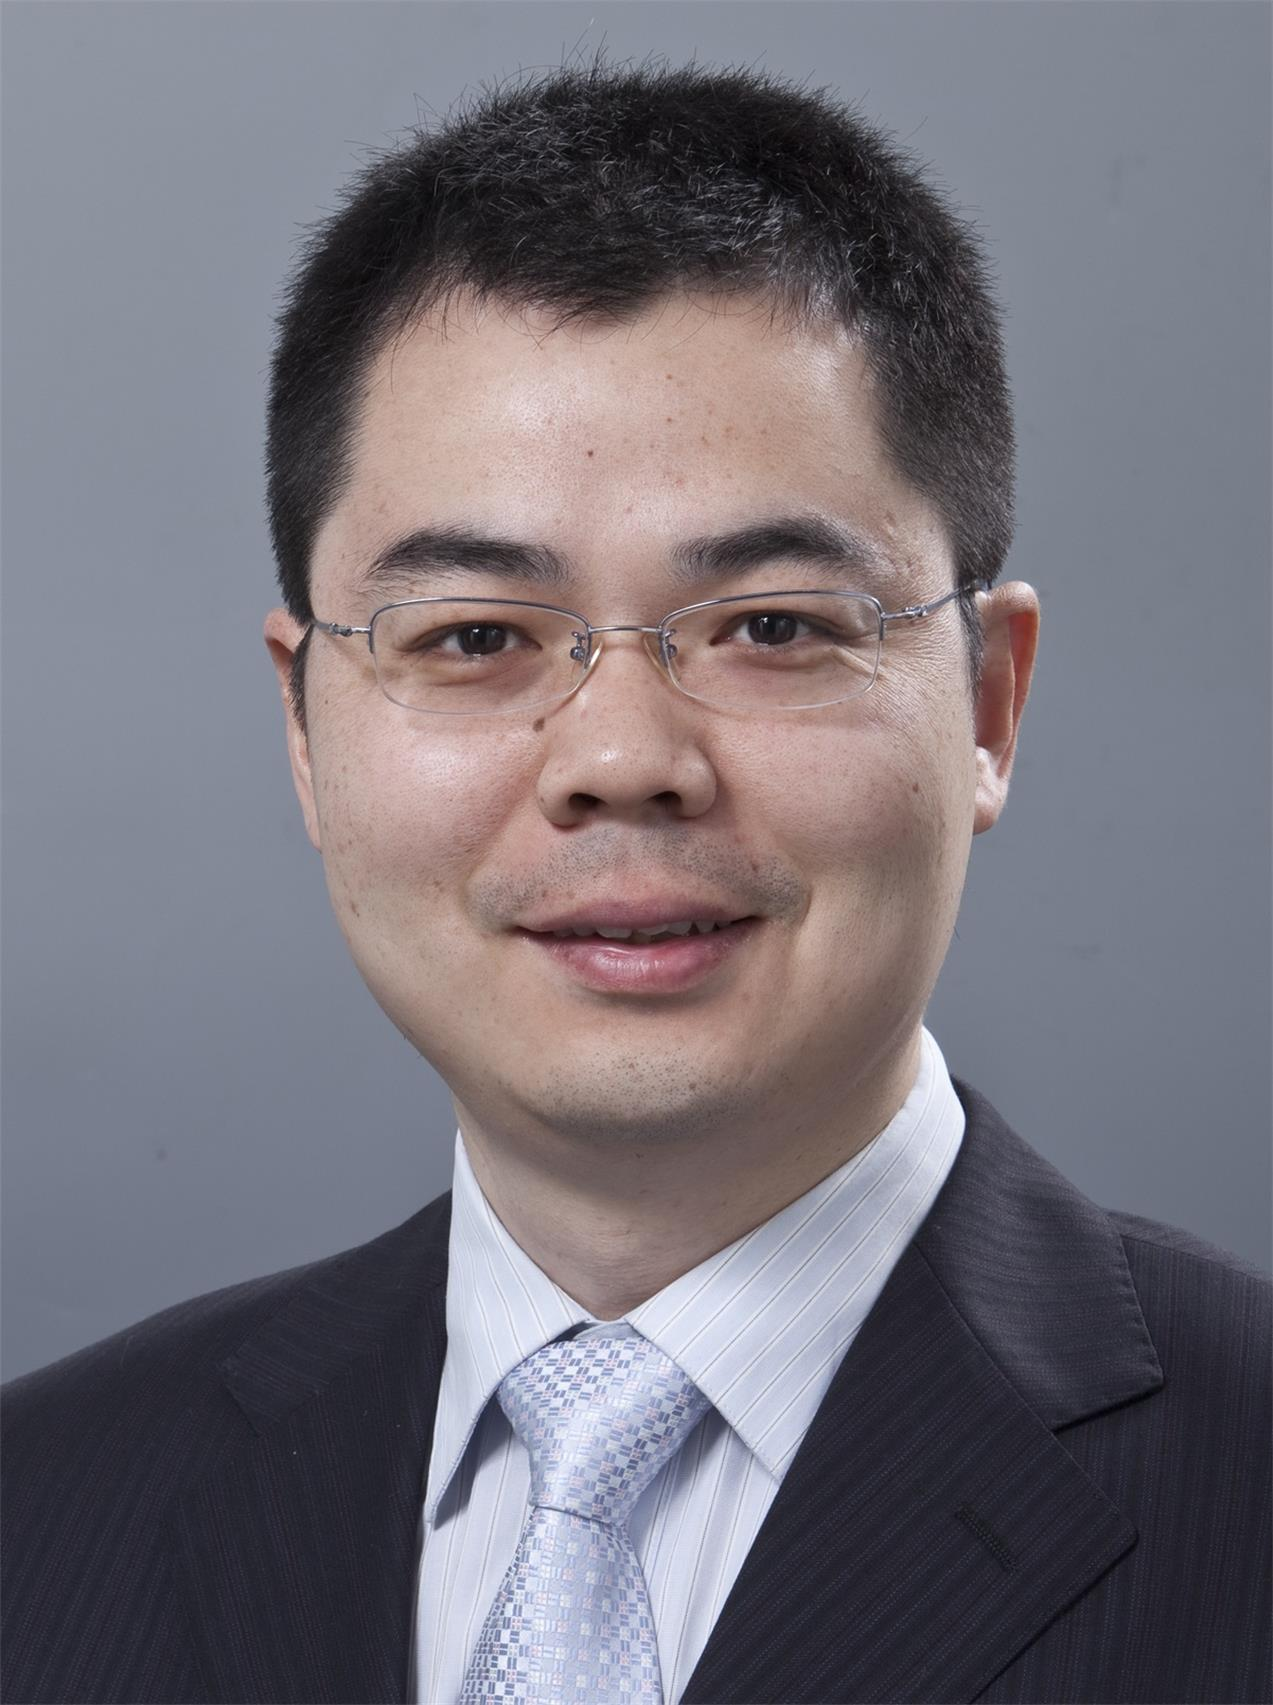
\includegraphics[width=1in,height
=1.25in,keepaspectratio]{Lei_Xie}}]{Lei Xie}
 received a B.S. degree in 2000 and a Ph.D. in 2005 from Zhejiang University, P.R. China. Between 2005 and 2006, he was a postdoctoral researcher at Berlin University of Technology, an Assistant Professor between 2005 and 2008 and is currently a Professor at the College of Control Science and Engineering, Zhejiang University. To date, his research activities culminated in over 40 articles that are published in internationally renowned journals and conferences, 3 book chapters and a book in the area of applied multivariate statistics and modeling. His research interests focus on the interdisciplinary area of statistics and system control theory.
\end{IEEEbiography}
\begin{IEEEbiography}[{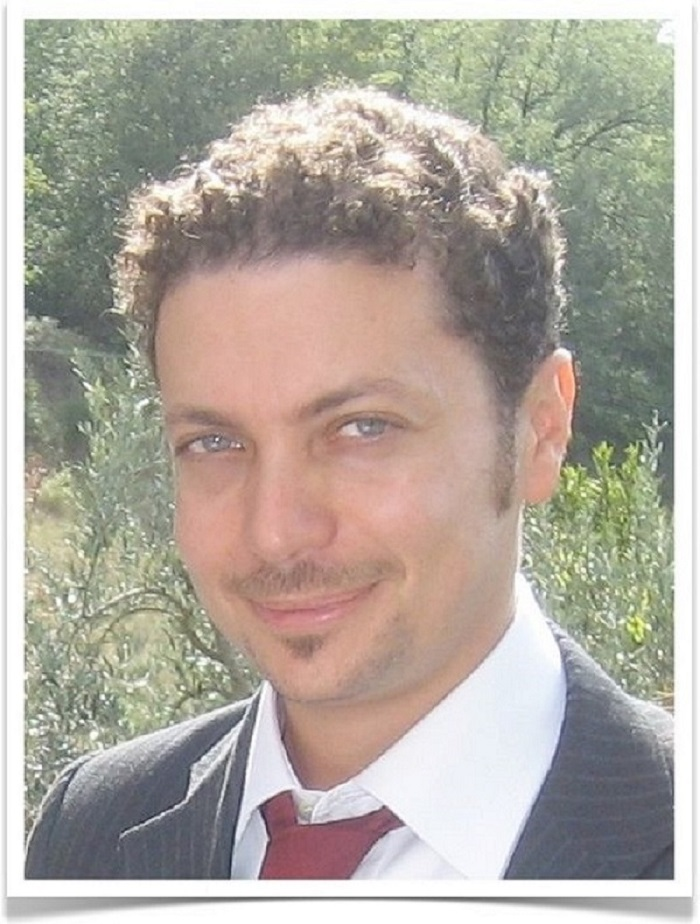
\includegraphics[width=1in,height
=1.25in,keepaspectratio]{Alberto_Bemporad}}]{Alberto Bemporad}received his master's degree in Electrical Engineering in 1993 and his Ph.D. in Control Engineering in 1997 from the University of Florence, Italy. In 1996/1997 he was with the Center for Robotics and Automation, Department of Systems Science \& Mathematics, Washington University, St. Louis. In 1997-1999 he held a postdoctoral position at the Automatic Control Laboratory, ETH Zurich, Switzerland, where he collaborated as a senior researcher until 2002. In 1999-2009 he was with the Department of Information Engineering of the University of Siena, Italy, becoming an associate professor in 2005. In 2010-2011 he was with the Department of Mechanical and Structural Engineering of the University of Trento, Italy. Since 2011 he is a full professor at the IMT School for Advanced Studies Lucca, Italy, where he served as the director of the institute in 2012-2015. He spent visiting periods at the University of Michigan, Zhejiang University, and Stanford University. In 2011 he cofounded ODYS S.r.l., a consulting and software development company specialized in advanced controls and embedded optimization algorithms. He has published more than 300 papers in the area of model predictive control, automotive control, hybrid systems, multiparametric optimization, computational geometry, robotics, and finance, and co-inventor of 8 patents. He is author or coauthor of various MATLAB toolboxes for model predictive control design, including the Model Predictive Control Toolbox and the Hybrid Toolbox. He was an Associate Editor of the IEEE Transactions on Automatic Control during 2001-2004 and Chair of the Technical Committee on Hybrid Systems of the IEEE Control Systems Society in 2002-2010. He received the IFAC High-Impact Paper Award for the 2011-2014 triennial. He has been an IEEE Fellow since 2010.
\end{IEEEbiography}


%\vfill

% Can be used to pull up biographies so that the bottom of the last one
% is flush with the other column.
%\enlargethispage{-5in}


%\end{spacing}{1.5}


% that's all folks
\end{document}


